\documentclass[aspectratio=169]{beamer}
\usepackage[preview]{cb-style}
\usepackage{mathtools}
%\usepackage{lmodern}
\usepackage{soul}
% \usepackage{enumitem}
\usepackage{multimedia}
\usepackage{hyperref}
\usepackage{adjustbox}
\usepackage{pgfplots}
\pgfplotsset{compat=1.17}
\usetikzlibrary{positioning, arrows.meta, fit, shapes.geometric, calc}

\newcommand{\numberset}{\mathbb}
\newcommand{\N}{\numberset{N}}
\newcommand{\Z}{\numberset{Z}}
\newcommand{\Q}{\numberset{Q}}
\newcommand{\R}{\numberset{R}}

\begin{document}
% Abstract of the talk at the end of the document

\begin{frame}
 \tableofcontents
\end{frame}

\section{Deep Learning}
\sectionpage

\begin{frame}{Regressione lineare}
    \begin{figure}
        \begin{minipage}{0.6\textwidth}
        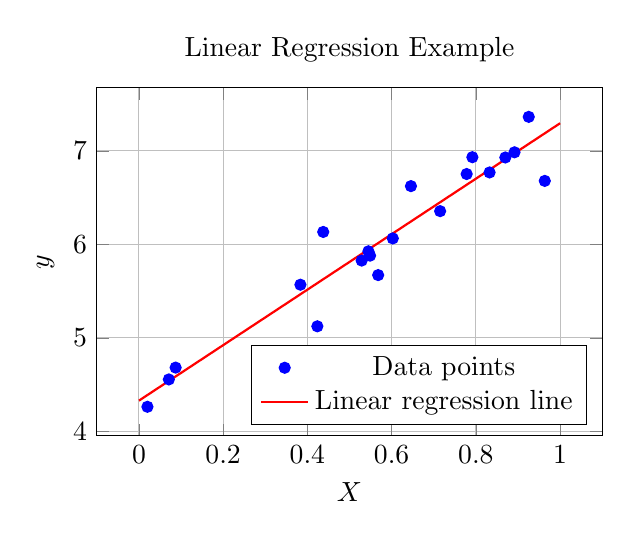
\begin{tikzpicture}
            \begin{axis}[
                width=8cm,
                height=6cm,
                xlabel={$X$},
                ylabel={$y$},
                title={Linear Regression Example},
                legend pos=south east,
                grid=major,
                ]
                % Data points
                \addplot[
                only marks,
                color=blue,
                mark=*,
                samples=100
                ] coordinates {
                    (0.5488135, 5.8798844)
                    (0.71518937, 6.3556331)
                    (0.60276338, 6.0641095)
                    (0.54488318, 5.926111)
                    (0.4236548, 5.124122)
                    (0.64589411, 6.6231887)
                    (0.43758721, 6.133222)
                    (0.891773, 6.984763)
                    (0.96366276, 6.678998)
                    (0.38344152, 5.568909)
                    (0.79172504, 6.932491)
                    (0.52889492, 5.827125)
                    (0.56804456, 5.671788)
                    (0.92559664, 7.363665)
                    (0.07103606, 4.556152)
                    (0.0871293, 4.682583)
                    (0.0202184, 4.263545)
                    (0.83261985, 6.769382)
                    (0.77815675, 6.752573)
                    (0.87001215, 6.929294)
                };
                
                % Linear regression line
                \addplot[
                color=red,
                thick
                ] coordinates {
                    (0, 4.3294)
                    (1, 1*2.9661+4.3294)
                };
                
                \legend{Data points, Linear regression line}
            \end{axis}
        \end{tikzpicture}
        \end{minipage}%
        \hfill
        \begin{minipage}{0.4\textwidth}
            Dove $\lbrace x_i \rbrace_{i}\subset \R$ sono i dati di input e $\lbrace y_i \rbrace_{i}\subset \R$ sono i dati di output. Noi vogliamo trovare la retta $y = w\cdot x + b$ che meglio approssima i dati.
        \end{minipage}
        \end{figure}  
\end{frame}

\begin{frame}{Regressione lineare}
    \begin{figure}
        \begin{minipage}{0.65\textwidth}
    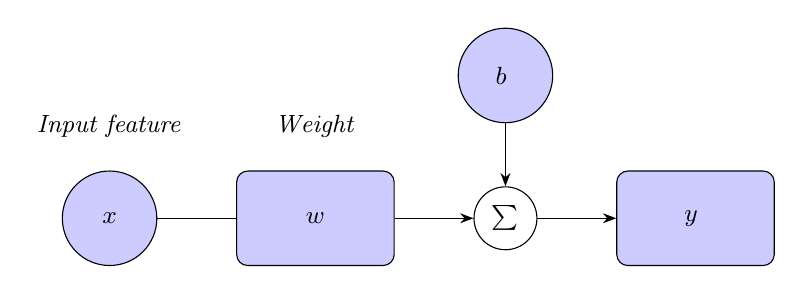
\begin{tikzpicture}
		\tikzset{
			>=Stealth,
			box/.style={draw, rounded corners, align=center, minimum height=1.2cm, minimum width=2cm, fill=blue!20},
			circlebox/.style={draw, circle, minimum size = 1.2cm, align=center, fill=blue!20},
			every node/.style={font=\small}
		}
		
		% Input nodes
		\node[circlebox] (x1) {$x$};
		
		% Weights and bias
		\node[box, right=1cm of x1] (w1) {$w$};
		
		% Sum node
		\node[draw, circle, fill=white, right=1cm of w1] (sum) { $\sum$ };
		
		% Output node
		\node[box, right=1cm of sum] (y) { $ y $ };
		
		% Bias node
		\node[circlebox, above=0.8cm of sum] (bias) { $ b $ };
		
		% Draw arrows between nodes
		\draw (x1) -- (w1);
		
		\draw[->] (w1) -- (sum);
		
		\draw[->] (bias) -- (sum);
		\draw[->] (sum) -- (y);
		
		% Annotations
		\node[above=0.3cm of w1] { \textit{Weight} };
		\node[above=0.3cm of x1] { \textit{Input feature} };
		
	\end{tikzpicture}
        \end{minipage}%
        \hfill
        \begin{minipage}{0.25\textwidth}
            \[y = w \cdot x + b\] 
            \begin{itemize}
            \item $x\in\R$ input,
            \item $w\in\R$ weight,
            \item $b\in\R$ bias.
            \end{itemize}        \end{minipage}
        \end{figure}  
\end{frame}


\begin{frame}{Regressione lineare}
    \begin{figure}
        \begin{minipage}{0.65\textwidth}
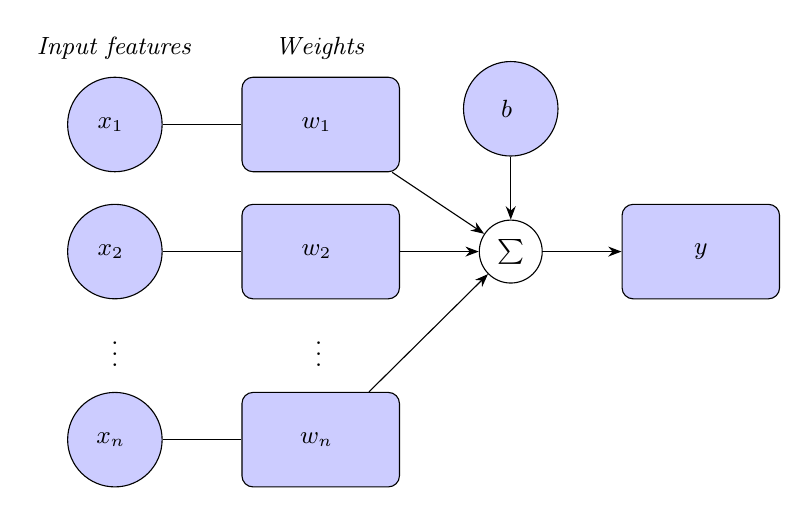
\begin{tikzpicture}
		\tikzset{
			>=Stealth,
			box/.style={draw, rounded corners, align=center, minimum height=1.2cm, minimum width=2cm, fill=blue!20},
			circlebox/.style={draw, circle, minimum size = 1.2cm, align=center, fill=blue!20},
			every node/.style={font=\small}
		}
		
		% Input nodes
		\node[circlebox] (x1) { \( x_1 \) };
		\node[circlebox, below=0.4cm of x1] (x2) { \( x_2 \) };
		\node[below=0.2cm of x2] (dots) { \vdots };
		\node[circlebox, below=0.2cm of dots] (xn) { \( x_n \) };
		
		% Weights and bias
		\node[box, right=1cm of x1] (w1) { \( w_1 \) };
		\node[box, right=1cm of x2] (w2) { \( w_2 \) };
        \node[right=2.25cm of dots] (dots_w) { \vdots };
		\node[box, right=1cm of xn] (wn) { \( w_n \) };
		
		% Sum node
		\node[draw, circle, fill=white, right=1cm of w2] (sum) { \( \sum \) };
		
		% Output node
		\node[box, right=1cm of sum] (y) {$y$};
		
		% Bias node
		\node[circlebox, above=0.8cm of sum] (bias) { \( b \) };
		
		% Draw arrows between nodes
		\draw (x1) -- (w1);
		\draw (x2) -- (w2);
		\draw (xn) -- (wn);
		
		\draw[->] (w1) -- (sum);
		\draw[->] (w2) -- (sum);
		\draw[->] (wn) -- (sum);
		
		\draw[->] (bias) -- (sum);
		\draw[->] (sum) -- (y);
		
		% Annotations
		\node[above=0.1cm of w1] { \textit{Weights} };
		\node[above=0.1cm of x1] { \textit{Input features} };
		
	\end{tikzpicture}
        \end{minipage}%
        \hfill
        \begin{minipage}{0.25\textwidth}
        \[y = \mathbf{w}\cdot \mathbf{x} + b\] 
        \begin{itemize}
        \item $\mathbf{x}\in\R^n$ inputs,
        \item $\mathbf{w}\in\R^n$ weights,
        \item $b\in\R$ bias.
        \end{itemize}
        \end{minipage}
        \end{figure}  
\end{frame}

\begin{frame}{Percettrone}
    \begin{figure}
        \begin{minipage}{0.6\textwidth}
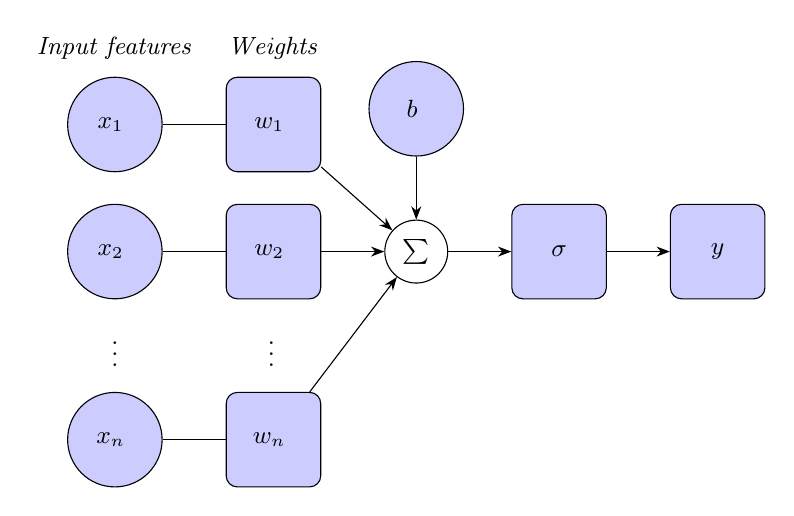
\begin{tikzpicture}
		\tikzset{
			>=Stealth,
			box/.style={draw, rounded corners, align=center, minimum height=1.2cm, minimum width=1.2cm, fill=blue!20},
			circlebox/.style={draw, circle, minimum size = 1.2cm, align=center, fill=blue!20},
			every node/.style={font=\small}
		}
		
		% Input nodes
		\node[circlebox] (x1) { \( x_1 \) };
		\node[circlebox, below=0.4cm of x1] (x2) { \( x_2 \) };
		\node[below=0.2cm of x2] (dots) { \vdots };
		\node[circlebox, below=0.2cm of dots] (xn) { \( x_n \) };
		
		% Weights and bias
		\node[box, right=0.8cm of x1] (w1) { \( w_1 \) };
		\node[box, right=0.8cm of x2] (w2) { \( w_2 \) };
        \node[right=1.65cm of dots] (dots_w) { \vdots };
		\node[box, right=0.8cm of xn] (wn) { \( w_n \) };
		
		% Sum node
		\node[draw, circle, fill=white, right=0.8cm of w2] (sum) { \( \sum \) };
		
		% activation
		\node[box, right=0.8cm of sum] (activation) {$\sigma$};

		% Output node
		\node[box, right=0.8cm of activation] (y) {$y$};
		
		% Bias node
		\node[circlebox, above=0.8cm of sum] (bias) { \( b \) };
		
		% Draw arrows between nodes
		\draw (x1) -- (w1);
		\draw (x2) -- (w2);
		\draw (xn) -- (wn);
		
		\draw[->] (w1) -- (sum);
		\draw[->] (w2) -- (sum);
		\draw[->] (wn) -- (sum);
		
		\draw[->] (bias) -- (sum);
		\draw[->] (sum) -- (activation);
        \draw[->] (activation) -- (y);
		
		% Annotations
		\node[above=0.1cm of w1] { \textit{Weights} };
		\node[above=0.1cm of x1] { \textit{Input features} };
		
	\end{tikzpicture}
        \end{minipage}%
        \hfill
        \begin{minipage}{0.3\textwidth}
        Problema di classificazione.
        \[y = \sigma\left(\mathbf{w}\cdot \mathbf{x} + b\right),\] 
        con $\sigma(z) = 1$ se $z\ge 0$ e nulla altrove.
        \end{minipage}
        \end{figure}  
\end{frame}

\begin{frame}{Percettrone}
    \begin{columns}
        \begin{column}{0.5\textwidth}
            Chiamiamo $\hat{y}(\mathbf{x})$ la label corretta associata ad $\mathbf{x}$, l'algoritmo per trovare $\mathbf{w}$ e $b$ \'e:
            \begin{itemize}
                \item calcolare $y(\mathbf{x}) = \sigma\left(\mathbf{w}\cdot \mathbf{x} + b\right) $, 
                \item se $y(\mathbf{x}) = \hat{y}(\mathbf{x})$ no aggiornamento,
                \item se $y(\mathbf{x})=1 $ e $\hat{y}(\mathbf{x}) = 0$ allora aggiorniamo $\mathbf{w} = \mathbf{w} + \eta \mathbf{x}$ e $b = b + \eta$.
                \item se $y(\mathbf{x})=0 $ e $\hat{y}(\mathbf{x}) = 1$ allora aggiorniamo $\mathbf{w} = \mathbf{w} - \eta \mathbf{x}$ e $b = b - \eta$.
            \end{itemize}
        \end{column}
        \pause
        \begin{column}{0.5\textwidth}
            \begin{center}
            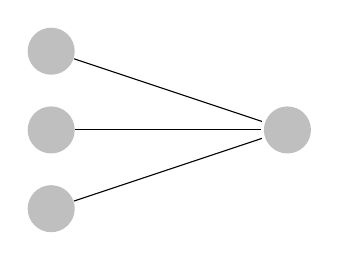
\begin{tikzpicture}[
                >=stealth,
                shorten >=1pt,
                auto,
                node distance=2cm,
                neuron/.style={circle, fill=black!25, minimum size=17pt, inner sep=0pt},
                layer/.style={thick, draw=black!50, rectangle, fill=black!10, minimum height=4em},
            ]
            
                % Draw the input layer nodes
                \foreach \name / \y in {1,...,3}
                    \node[neuron] (I-\name) at (0,-\y) {};
            
                % Draw the output layer node
                \foreach \name / \y in {2}
                    \node[neuron] (O-\name) at (3,-\y) {};
            
                % Connect every node in the input layer with every node in the
                % hidden layer.
                \foreach \source in {1,...,3}
                    \foreach \dest in {2}
                        \path (I-\source) edge (O-\dest);
            \end{tikzpicture}%
            \end{center}
            Ogni freccia rappresenta una connessione a cui è associato un peso, ed ogni cerchio rappresenta un neurone, a cui è associato un bias.
        \end{column}
    \end{columns}
\end{frame}

\begin{frame}{Percettrone}
Notiamo che se $x_{0}, x_{1} \in \lbrace 0, 1 \rbrace$ allora con il percettrone si puo' rappresentare le operazioni logiche di negazione, congiunzione e disgiunzione.
\begin{figure}
    \centering
    \begin{minipage}{0.3\textwidth}
        \begin{center}
            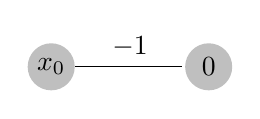
\begin{tikzpicture}[
                >=stealth,
                shorten >=1pt,
                auto,
                node distance=2cm,
                neuron/.style={circle, fill=black!25, minimum size=17pt, inner sep=0pt},
                layer/.style={thick, draw=black!50, rectangle, fill=black!10, minimum height=4em},
            ]
                % Draw the input layer nodes
                \foreach \name / \y in {0}
                    \node[neuron, align=center] (I-\name) at (0,-\y) {$x_{\y }$};

                % Draw the output layer node
                \foreach \name / \y in {0}
                    \node[neuron, align=center] (O-\name) at (2, -\y) {$0$};

                % Connect every node in the input layer with every node in the
                % hidden layer.
                \foreach \source in {0}
                    \foreach \dest in {0}
                        \path (I-\source) edge node[midway, above, sloped] {$-1$} (O-\dest);
            \end{tikzpicture}%
        \end{center}
        \caption{Negazione}
    \end{minipage}%
    \hfill
    \begin{minipage}{0.3\textwidth}
        \begin{center}
            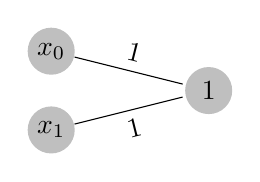
\begin{tikzpicture}[
                >=stealth,
                shorten >=1pt,
                auto,
                node distance=2cm,
                neuron/.style={circle, fill=black!25, minimum size=17pt, inner sep=0pt},
                layer/.style={thick, draw=black!50, rectangle, fill=black!10, minimum height=4em},
            ]
                % Draw the input layer nodes
                \foreach \name / \y in {0,1}
                    \node[neuron, align=center] (I-\name) at (0,-\y) {$x_{\y }$};

                % Draw the output layer node
                \foreach \name / \y in {0}
                    \node[neuron, align=center] (O-\name) at (2, -0.5-\y) {$1$};

                % Connect every node in the input layer with every node in the
                % hidden layer.
                \foreach \source in {0}
                    \foreach \dest in {0}
                        \path (I-\source) edge node[midway, above, sloped] {$1$} (O-\dest);
                \foreach \source in {1}
                    \foreach \dest in {0}
                        \path (I-\source) edge node[midway, below, sloped] {$1$} (O-\dest);
            \end{tikzpicture}%
        \end{center}
        \caption{Congiunzione}
    \end{minipage}%
    \hfill
    \begin{minipage}{0.3\textwidth}
        \begin{center}
            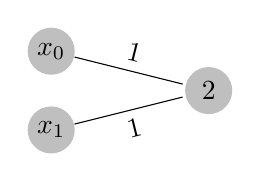
\begin{tikzpicture}[
                >=stealth,
                shorten >=1pt,
                auto,
                node distance=2cm,
                neuron/.style={circle, fill=black!25, minimum size=17pt, inner sep=0pt},
                layer/.style={thick, draw=black!50, rectangle, fill=black!10, minimum height=4em},
            ]
                % Draw the input layer nodes
                \foreach \name / \y in {0,1}
                    \node[neuron, align=center] (I-\name) at (0,-\y) {$x_{\y }$};

                % Draw the output layer node
                \foreach \name / \y in {0}
                    \node[neuron, align=center] (O-\name) at (2, -0.5-\y) {$2$};

                % Connect every node in the input layer with every node in the
                % hidden layer.
                \foreach \source in {0}
                    \foreach \dest in {0}
                        \path (I-\source) edge node[midway, above, sloped] {$1$} (O-\dest);
                \foreach \source in {1}
                    \foreach \dest in {0}
                        \path (I-\source) edge node[midway, below, sloped] {$1$} (O-\dest);
            \end{tikzpicture}%
        \end{center}
        \caption{Disgiunzione}
    \end{minipage}
\end{figure}

\pause
Ma non si puo' rappresentare la disgiunzione esclusiva (XOR).
\end{frame}

\begin{frame}{Multi-layer Perceptron}
    Indicando lo XOR con $\times$ vale che
    \[
    x_{1} \times x_{2} = (x_{1} \lor x_{2}) \land \neg (x_{1} \land x_{2}) = (x_{1} \lor x_{2}) \land (\neg x_{1} \lor \neg x_{2}).
    \]
    \pause
    Dunque lo possiamo rappresentare con
    \begin{center}
        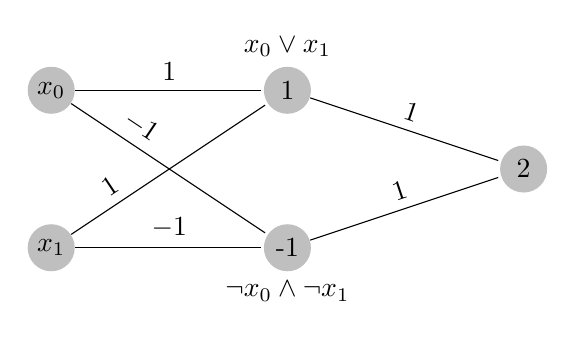
\begin{tikzpicture}[
            >=stealth,
            shorten >=1pt,
            auto,
            node distance=2cm,
            neuron/.style={circle, fill=black!25, minimum size=17pt, inner sep=0pt},
            layer/.style={thick, draw=black!50, rectangle, fill=black!10, minimum height=4em},
        ]
            % Draw the input layer nodes
            \foreach \name / \y in {0,1}
                \node[neuron, align=center] (I-\name) at (0,-2*\y) {$x_{\y}$};

            % Draw the hidden layer nodes
            \foreach \name / \y in {0}
                \node[neuron, align=center, label=above:{$x_{0} \lor x_{1}$}] (H-\name) at (3,-2*\y) {1};
            \foreach \name / \y in {1}
                \node[neuron, align=center, label=below:{$\neg x_{0} \land \neg x_{1}$}] (H-\name) at (3,-2*\y) {-1};

            % Draw the output layer node
            \foreach \name / \y in {0}
                \node[neuron, align=center] (O-\name) at (6, -1-\y) {$2$};

            % Connect every node in the input layer with every node in the
            % hidden layer.
            \path (I-0) edge node[midway, above, sloped] {$1$} (H-0);
            \path (I-0) edge node[pos=0.3, above, sloped] {$-1$} (H-1);
            \path (I-1) edge node[pos=0.25, above, sloped] {$1$} (H-0);
            \path (I-1) edge node[midway, above, sloped] {$-1$} (H-1);

            \path (H-0) edge node[midway, above, sloped] {$1$} (O-0);
            \path (H-1) edge node[midway, above, sloped] {$1$} (O-0);
        \end{tikzpicture}%
    \end{center}
\end{frame}

\begin{frame}{Multi-layer Perceptron}
    \begin{figure}
        \begin{minipage}{0.65\textwidth}
    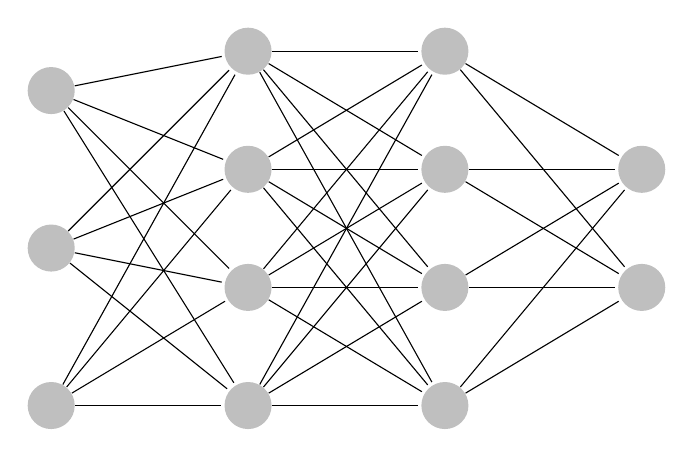
\begin{tikzpicture}[
        >=stealth,
        shorten >=1pt,
        auto,
        node distance=2cm,
        neuron/.style={circle, fill=black!25, minimum size=17pt, inner sep=0pt},
        layer/.style={thick, draw=black!50, rectangle, fill=black!10, minimum height=4em},
    ]
    
        % Draw the input layer nodes
        \foreach \name / \y in {1,...,3}
            \node[neuron] (I-\name) at (0,-\y*2) {};
    
        % Draw the hidden layer nodes
        \foreach \name / \y in {1,...,4}
            \node[neuron] (H1-\name) at (2.5,-\y*1.5) {};
            
        \foreach \name / \y in {1,...,4}
            \node[neuron] (H2-\name) at (5,-\y*1.5) {};
    
        % Draw the output layer node
        \foreach \name / \y in {2,3}
            \node[neuron] (O-\name) at (7.5,-\y*1.5) {};
    
        % Connect every node in the input layer with every node in the
        % hidden layer.
        \foreach \source in {1,...,3}
            \foreach \dest in {1,...,4}
                \path (I-\source) edge (H1-\dest);
                
        \foreach \source in {1,...,4}
            \foreach \dest in {1,...,4}
                \path (H1-\source) edge (H2-\dest);
    
        % Connect every node in the hidden layer with the output layer
        \foreach \source in {1,...,4}
            \foreach \dest in {2,3}
                \path (H2-\source) edge (O-\dest);
    \end{tikzpicture}%
        \end{minipage}%
        \hfill
        \begin{minipage}{0.35\textwidth}
        Esempio di architettura di un Multi-layer Perceptron con $3$ neuroni di input, $4$ neuroni nel primo hidden layer, $4$ neuroni nel secondo hidden layer e $2$ neuroni di output.
        \end{minipage}
        \end{figure}  
\end{frame}

\begin{frame}{Multi-layer Perceptron}
    \begin{figure}
        \begin{minipage}{0.65\textwidth}
    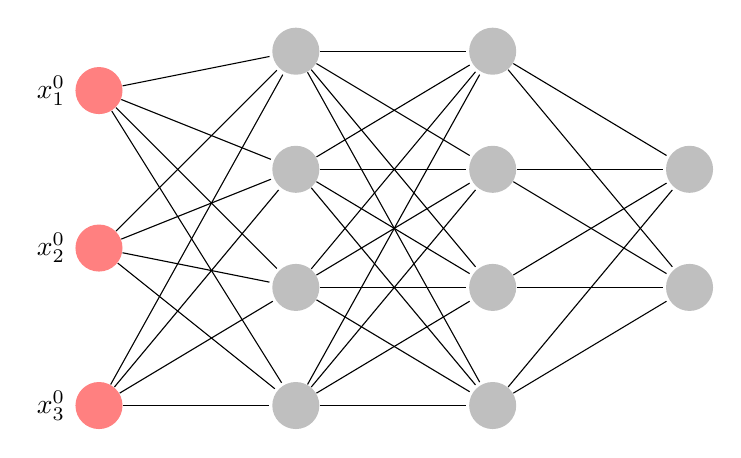
\begin{tikzpicture}[
        >=stealth,
        shorten >=1pt,
        auto,
        node distance=2cm,
        neuron/.style={circle, fill=black!25, minimum size=17pt, inner sep=0pt},
        layer/.style={thick, draw=black!50, rectangle, fill=black!10, minimum height=4em},
    ]
    
        % Draw the input layer nodes
        \foreach \name / \y in {1,...,3}
            \node[neuron, fill=red!50, label=left:{$x_{\name}^{0}$}] (I-\name) at (0,-\y*2) {};
    
        % Draw the hidden layer nodes
        \foreach \name / \y in {1,...,4}
            \node[neuron] (H1-\name) at (2.5,-\y*1.5) {};
            
        \foreach \name / \y in {1,...,4}
            \node[neuron] (H2-\name) at (5,-\y*1.5) {};
    
        % Draw the output layer node
        \foreach \name / \y in {2,3}
            \node[neuron] (O-\name) at (7.5,-\y*1.5) {};
    
        % Connect every node in the input layer with every node in the
        % hidden layer.
        \foreach \source in {1,...,3}
            \foreach \dest in {1,...,4}
                \path (I-\source) edge (H1-\dest);
                
        \foreach \source in {1,...,4}
            \foreach \dest in {1,...,4}
                \path (H1-\source) edge (H2-\dest);
    
        % Connect every node in the hidden layer with the output layer
        \foreach \source in {1,...,4}
            \foreach \dest in {2,3}
                \path (H2-\source) edge (O-\dest);
            \end{tikzpicture}%
        \end{minipage}%
        \hfill
        \begin{minipage}{0.35\textwidth}
            Layer di input con $3$ neuroni.
        \end{minipage}
        \end{figure}  
\end{frame}

\begin{frame}{Multi-layer Perceptron}
    \begin{figure}
        \begin{minipage}{0.65\textwidth}
    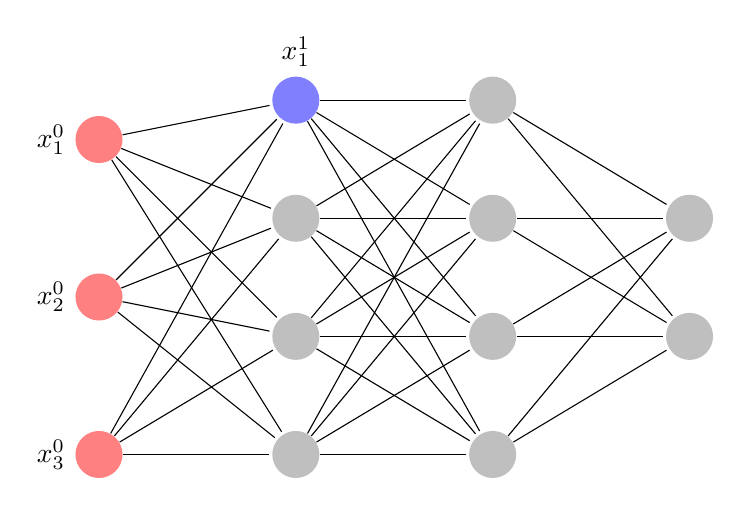
\begin{tikzpicture}[
        >=stealth,
        shorten >=1pt,
        auto,
        node distance=2cm,
        neuron/.style={circle, fill=black!25, minimum size=17pt, inner sep=0pt},
        layer/.style={thick, draw=black!50, rectangle, fill=black!10, minimum height=4em},
    ]
    
        % Draw the input layer nodes
        \foreach \name / \y in {1,...,3}
            \node[neuron, fill=red!50, label=left:{$x_{\name}^{0}$}] (I-\name) at (0,-\y*2) {};
    
        % Draw the hidden layer nodes
        \foreach \name / \y in {1}
            \node[neuron, fill=blue!50, label=above:{$x_{\name}^{1}$}] (H1-\name) at (2.5,-\y*1.5) {};
        \foreach \name / \y in {2,...,4}
            \node[neuron] (H1-\name) at (2.5,-\y*1.5) {};
            
        \foreach \name / \y in {1,...,4}
            \node[neuron] (H2-\name) at (5,-\y*1.5) {};
    
        % Draw the output layer node
        \foreach \name / \y in {2,3}
            \node[neuron] (O-\name) at (7.5,-\y*1.5) {};
    
        % Connect every node in the input layer with every node in the
        % hidden layer.
        \foreach \source in {1,...,3}
            \foreach \dest in {1,...,4}
                \path (I-\source) edge (H1-\dest);
                
        \foreach \source in {1,...,4}
            \foreach \dest in {1,...,4}
                \path (H1-\source) edge (H2-\dest);
    
        % Connect every node in the hidden layer with the output layer
        \foreach \source in {1,...,4}
            \foreach \dest in {2,3}
                \path (H2-\source) edge (O-\dest);
            \end{tikzpicture}%
        \end{minipage}%
        \hfill
        \begin{minipage}{0.35\textwidth}
        Vogliamo definire il valore del neurone $x_{1}^{1}$.
        \end{minipage}
        \end{figure}  
\end{frame}

\begin{frame}{Multi-layer Perceptron}
    \begin{figure}
        \begin{minipage}{0.65\textwidth}
    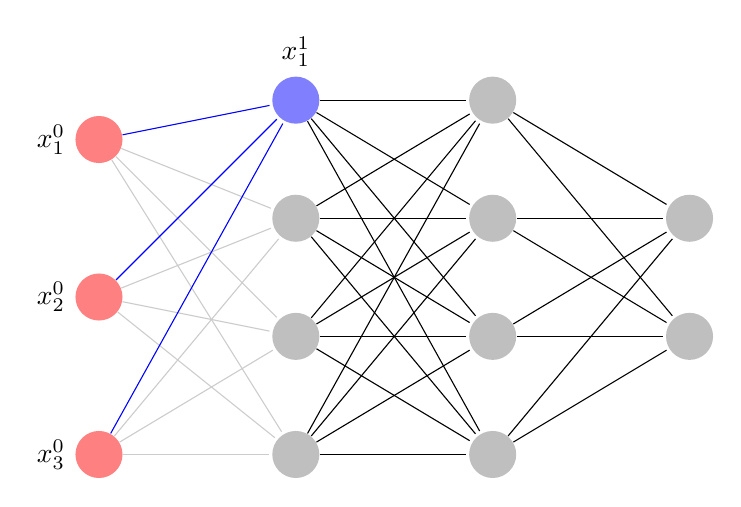
\begin{tikzpicture}[
        >=stealth,
        shorten >=1pt,
        auto,
        node distance=2cm,
        neuron/.style={circle, fill=black!25, minimum size=17pt, inner sep=0pt},
        layer/.style={thick, draw=black!50, rectangle, fill=black!10, minimum height=4em},
    ]
    
        % Draw the input layer nodes
        \foreach \name / \y in {1,...,3}
            \node[neuron, fill=red!50, label=left:{$x_{\name}^{0}$}] (I-\name) at (0,-\y*2) {};
    
        % Draw the hidden layer nodes
        \foreach \name / \y in {1}
            \node[neuron, fill=blue!50, label=above:{$x_{\name}^{1}$}] (H1-\name) at (2.5,-\y*1.5) {};
        \foreach \name / \y in {2,...,4}
            \node[neuron] (H1-\name) at (2.5,-\y*1.5) {};
            
        \foreach \name / \y in {1,...,4}
            \node[neuron] (H2-\name) at (5,-\y*1.5) {};
    
        % Draw the output layer node
        \foreach \name / \y in {2,3}
            \node[neuron] (O-\name) at (7.5,-\y*1.5) {};
    
        % Connect every node in the input layer with every node in the
        % hidden layer.
        \foreach \source in {1,...,3}
            \foreach \dest in {2, ..., 4}
                \path (I-\source) edge[draw=black!20] (H1-\dest);
        \foreach \source in {1,...,3}
            \foreach \dest in {1}
				\path (I-\source) edge[draw=blue] (H1-\dest); 
                
        \foreach \source in {1,...,4}
            \foreach \dest in {1,...,4}
                \path (H1-\source) edge (H2-\dest);
    
        % Connect every node in the hidden layer with the output layer
        \foreach \source in {1,...,4}
            \foreach \dest in {2,3}
                \path (H2-\source) edge (O-\dest);
            \end{tikzpicture}%
        \end{minipage}%
        \hfill
        \begin{minipage}{0.35\textwidth}
        Evidenziamo le connesioni con i neuroni nel layer precedente.
        \end{minipage}
        \end{figure}  
\end{frame}

\begin{frame}{Multi-layer Perceptron}
    \begin{figure}
        \begin{minipage}{0.65\textwidth}
    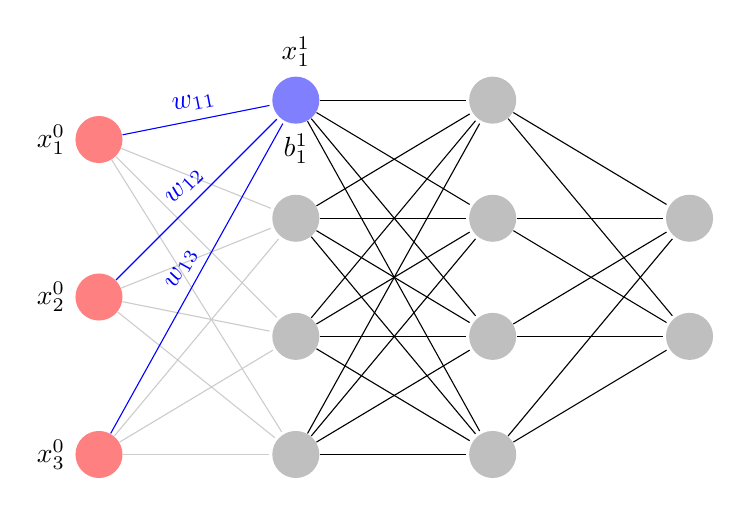
\begin{tikzpicture}[
        >=stealth,
        shorten >=1pt,
        auto,
        node distance=2cm,
        neuron/.style={circle, fill=black!25, minimum size=17pt, inner sep=0pt},
        layer/.style={thick, draw=black!50, rectangle, fill=black!10, minimum height=4em},
    ]
    
        % Draw the input layer nodes
        \foreach \name / \y in {1,...,3}
            \node[neuron, fill=red!50, label=left:{$x_{\name}^{0}$}] (I-\name) at (0,-\y*2) {};
    
        % Draw the hidden layer nodes
        \foreach \name / \y in {1}
			\node[neuron, fill=blue!50, label=above:{$x_{\name}^{1}$}, label=below:{$b_{\name}^{1}$}] (H1-\name) at (2.5,-\y*1.5) {};
        \foreach \name / \y in {2,...,4}
            \node[neuron] (H1-\name) at (2.5,-\y*1.5) {};
            
        \foreach \name / \y in {1,...,4}
            \node[neuron] (H2-\name) at (5,-\y*1.5) {};
    
        % Draw the output layer node
        \foreach \name / \y in {2,3}
            \node[neuron] (O-\name) at (7.5,-\y*1.5) {};
    
        % Connect every node in the input layer with every node in the
        % hidden layer.
        \foreach \source in {1,...,3}
            \foreach \dest in {2, ..., 4}
                \path (I-\source) edge[draw=black!20] (H1-\dest);
        \foreach \source in {1,...,3}
            \foreach \dest in {1}
				\path (I-\source) edge[draw=blue] node[midway, above, sloped, text=blue] {$w_{\dest\source}$} (H1-\dest); 
                
        \foreach \source in {1,...,4}
            \foreach \dest in {1,...,4}
                \path (H1-\source) edge (H2-\dest);
    
        % Connect every node in the hidden layer with the output layer
        \foreach \source in {1,...,4}
            \foreach \dest in {2,3}
                \path (H2-\source) edge (O-\dest);
    \end{tikzpicture}%
\end{minipage}%
\hfill
\begin{minipage}{0.35\textwidth}
    \[x_{1}^{1} = \sigma\left( b_{1}^{1} + \sum_{i=1}^{3} w_{1i}x_{i}^{0}\right)\]
    Dove $\sigma$ è una funzione di attivazione non lineare.
\end{minipage}
\end{figure}  
\end{frame}


\begin{frame}{Multi-layer Perceptron}
    \begin{figure}
        \begin{minipage}{0.65\textwidth}
    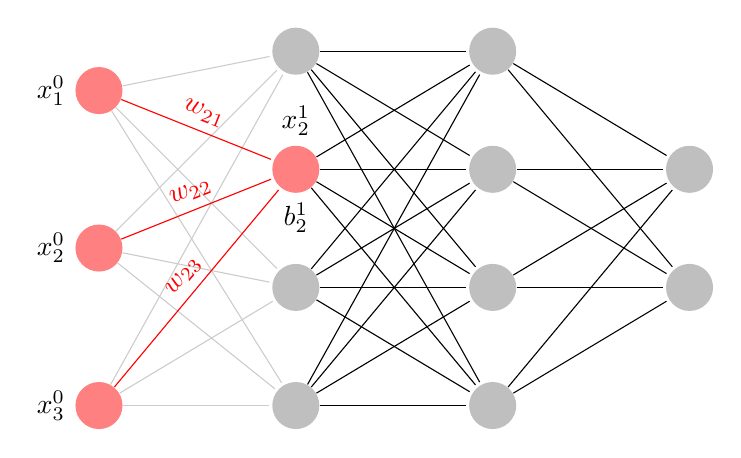
\begin{tikzpicture}[
        >=stealth,
        shorten >=1pt,
        auto,
        node distance=2cm,
        neuron/.style={circle, fill=black!25, minimum size=17pt, inner sep=0pt},
        layer/.style={thick, draw=black!50, rectangle, fill=black!10, minimum height=4em},
    ]
    
        % Draw the input layer nodes
        \foreach \name / \y in {1,...,3}
            \node[neuron, fill=red!50, label=left:{$x_{\name}^{0}$}] (I-\name) at (0,-\y*2) {};
    
        % Draw the hidden layer nodes
        \foreach \name / \y in {2}
			\node[neuron, fill=red!50, label=above:{$x_{\name}^{1}$}, label=below:{$b_{\name}^{1}$}] (H1-\name) at (2.5,-\y*1.5) {};
        \foreach \name / \y in {1, 3, 4}
            \node[neuron] (H1-\name) at (2.5,-\y*1.5) {};
            
        \foreach \name / \y in {1,...,4}
            \node[neuron] (H2-\name) at (5,-\y*1.5) {};
    
        % Draw the output layer node
        \foreach \name / \y in {2,3}
            \node[neuron] (O-\name) at (7.5,-\y*1.5) {};
    
        % Connect every node in the input layer with every node in the
        % hidden layer.
        \foreach \source in {1,...,3}
            \foreach \dest in {1, 3, 4}
                \path (I-\source) edge[draw=black!20] (H1-\dest);
        \foreach \source in {1,...,3}
            \foreach \dest in {2}
				\path (I-\source) edge[draw=red] node[midway, above, sloped, text=red] {$w_{\dest\source}$} (H1-\dest); 
                
        \foreach \source in {1,...,4}
            \foreach \dest in {1,...,4}
                \path (H1-\source) edge (H2-\dest);
    
        % Connect every node in the hidden layer with the output layer
        \foreach \source in {1,...,4}
            \foreach \dest in {2,3}
                \path (H2-\source) edge (O-\dest);
    \end{tikzpicture}%
\end{minipage}%
\hfill
\begin{minipage}{0.35\textwidth}
    \[x_{1}^{1} = \sigma\left(b_{1}^{1} +\sum_{i=1}^{3} w_{1i}x_{i}^{0} \right) \]
    \[x_{2}^{1} = \sigma\left( b_{2}^{1}+\sum_{i=1}^{4} w_{2i}x_{i}^{0} \right) \]
\end{minipage}
\end{figure}  
\end{frame}


\begin{frame}{Multi-layer Perceptron}
    \begin{figure}
        \begin{minipage}{0.65\textwidth}
    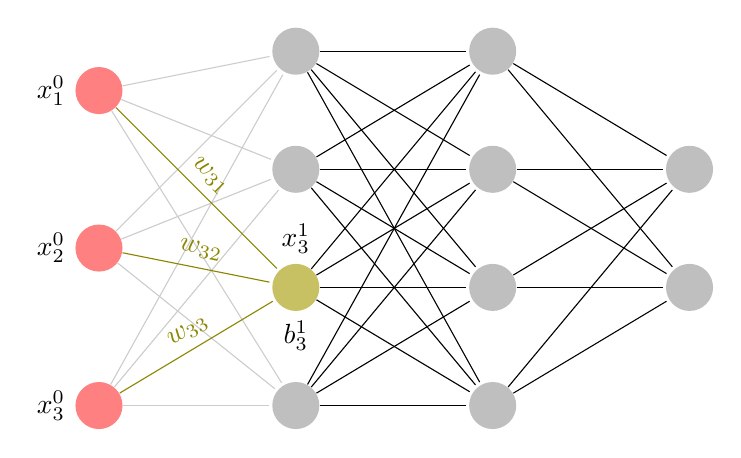
\begin{tikzpicture}[
        >=stealth,
        shorten >=1pt,
        auto,
        node distance=2cm,
        neuron/.style={circle, fill=black!25, minimum size=17pt, inner sep=0pt},
        layer/.style={thick, draw=black!50, rectangle, fill=black!10, minimum height=4em},
    ]
    
        % Draw the input layer nodes
        \foreach \name / \y in {1,...,3}
            \node[neuron, fill=red!50, label=left:{$x_{\name}^{0}$}] (I-\name) at (0,-\y*2) {};
    
        % Draw the hidden layer nodes
        \foreach \name / \y in {3}
			\node[neuron, fill=olive!50, label=above:{$x_{\name}^{1}$}, label=below:{$b_{\name}^{1}$}] (H1-\name) at (2.5,-\y*1.5) {};
        \foreach \name / \y in {1, 2, 4}
            \node[neuron] (H1-\name) at (2.5,-\y*1.5) {};
            
        \foreach \name / \y in {1,...,4}
            \node[neuron] (H2-\name) at (5,-\y*1.5) {};
    
        % Draw the output layer node
        \foreach \name / \y in {2,3}
            \node[neuron] (O-\name) at (7.5,-\y*1.5) {};
    
        % Connect every node in the input layer with every node in the
        % hidden layer.
        \foreach \source in {1,...,3}
            \foreach \dest in {1, 2, 4}
                \path (I-\source) edge[draw=black!20] (H1-\dest);
        \foreach \source in {1,...,3}
            \foreach \dest in {3}
				\path (I-\source) edge[draw=olive] node[midway, above, sloped, text=olive] {$w_{\dest\source}$} (H1-\dest); 
                
        \foreach \source in {1,...,4}
            \foreach \dest in {1,...,4}
                \path (H1-\source) edge (H2-\dest);
    
        % Connect every node in the hidden layer with the output layer
        \foreach \source in {1,...,4}
            \foreach \dest in {2,3}
                \path (H2-\source) edge (O-\dest);
    \end{tikzpicture}%
\end{minipage}%
\hfill
\begin{minipage}{0.35\textwidth}
    \[x_{1}^{1} = \sigma\left(b_{1}^{1}+\sum_{i=1}^{3} w_{1i}x_{i}^{0} \right) \]
    \[x_{2}^{1} = \sigma\left(b_{2}^{1}+\sum_{i=1}^{4} w_{2i}x_{i}^{0} \right) \]
    \[x_{3}^{1} = \sigma\left(b_{3}^{1}+\sum_{i=1}^{4} w_{3i}x_{i}^{0} \right) \]
\end{minipage}
\end{figure}  
\end{frame}


\begin{frame}{Multi-layer Perceptron}
    \begin{figure}
        \begin{minipage}{0.65\textwidth}
    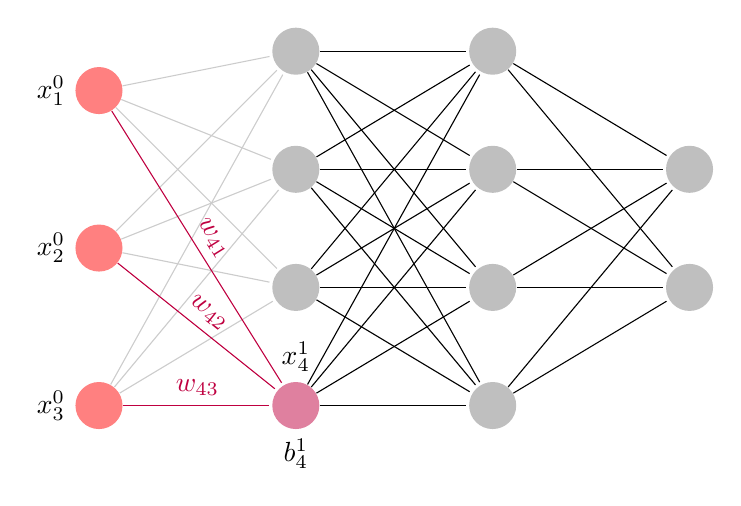
\begin{tikzpicture}[
        >=stealth,
        shorten >=1pt,
        auto,
        node distance=2cm,
        neuron/.style={circle, fill=black!25, minimum size=17pt, inner sep=0pt},
        layer/.style={thick, draw=black!50, rectangle, fill=black!10, minimum height=4em},
    ]
    
        % Draw the input layer nodes
        \foreach \name / \y in {1,...,3}
            \node[neuron, fill=red!50, label=left:{$x_{\name}^{0}$}] (I-\name) at (0,-\y*2) {};
    
        % Draw the hidden layer nodes
        \foreach \name / \y in {4}
			\node[neuron, fill=purple!50, label=above:{$x_{\name}^{1}$}, label=below:{$b_{\name}^{1}$}] (H1-\name) at (2.5,-\y*1.5) {};
        \foreach \name / \y in {1, ..., 3}
            \node[neuron] (H1-\name) at (2.5,-\y*1.5) {};
            
        \foreach \name / \y in {1,...,4}
            \node[neuron] (H2-\name) at (5,-\y*1.5) {};
    
        % Draw the output layer node
        \foreach \name / \y in {2,3}
            \node[neuron] (O-\name) at (7.5,-\y*1.5) {};
    
        % Connect every node in the input layer with every node in the
        % hidden layer.
        \foreach \source in {1,...,3}
            \foreach \dest in {1, ..., 3}
                \path (I-\source) edge[draw=black!20] (H1-\dest);
        \foreach \source in {1,...,3}
            \foreach \dest in {4}
				\path (I-\source) edge[draw=purple] node[midway, above, sloped, text=purple] {$w_{\dest\source}$} (H1-\dest); 
                
        \foreach \source in {1,...,4}
            \foreach \dest in {1,...,4}
                \path (H1-\source) edge (H2-\dest);
    
        % Connect every node in the hidden layer with the output layer
        \foreach \source in {1,...,4}
            \foreach \dest in {2,3}
                \path (H2-\source) edge (O-\dest);
    \end{tikzpicture}%
\end{minipage}%
\hfill
\begin{minipage}{0.35\textwidth}
    \vspace{-1cm}
    \[x_{1}^{1} = \sigma\left(b_{1}^{1}+\sum_{i=1}^{3} w_{1i}x_{i}^{0} \right) \]
    \[x_{2}^{1} = \sigma\left(b_{2}^{1}+\sum_{i=1}^{4} w_{2i}x_{i}^{0} \right) \]
    \[x_{3}^{1} = \sigma\left(b_{3}^{1}+\sum_{i=1}^{4} w_{3i}x_{i}^{0} \right) \]
    \[x_{4}^{1} = \sigma\left(b_{4}^{1}+\sum_{i=1}^{2} w_{4i}x_{i}^{0} \right) \]
\end{minipage}
\end{figure}  
\end{frame}


\begin{frame}{Multi-layer Perceptron}
    \begin{figure}
        \begin{minipage}{0.65\textwidth}
    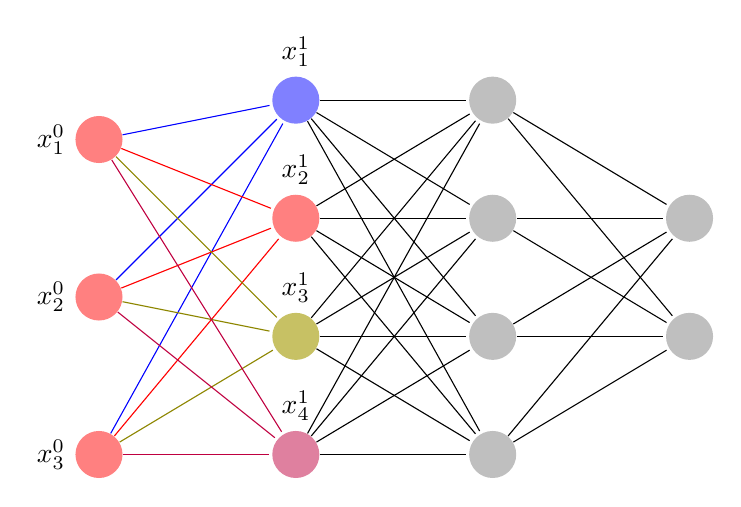
\begin{tikzpicture}[
        >=stealth,
        shorten >=1pt,
        auto,
        node distance=2cm,
        neuron/.style={circle, fill=black!25, minimum size=17pt, inner sep=0pt},
        layer/.style={thick, draw=black!50, rectangle, fill=black!10, minimum height=4em},
    ]
    
        % Draw the input layer nodes
        \foreach \name / \y in {1,...,3}
            \node[neuron, fill=red!50, label=left:{$x_{\name}^{0}$}] (I-\name) at (0,-\y*2) {};
    
        % Draw the hidden layer nodes
        \foreach \name / \y in {1}
			\node[neuron, fill=blue!50, label=above:{$x_{\name}^{1}$}] (H1-\name) at (2.5,-\y*1.5) {};
        \foreach \name / \y in {2}
			\node[neuron, fill=red!50, label=above:{$x_{\name}^{1}$}] (H1-\name) at (2.5,-\y*1.5) {};
        \foreach \name / \y in {3}
			\node[neuron, fill=olive!50, label=above:{$x_{\name}^{1}$}] (H1-\name) at (2.5,-\y*1.5) {};
        \foreach \name / \y in {4}
			\node[neuron, fill=purple!50, label=above:{$x_{\name}^{1}$}] (H1-\name) at (2.5,-\y*1.5) {};
            
        \foreach \name / \y in {1,...,4}
            \node[neuron] (H2-\name) at (5,-\y*1.5) {};
    
        % Draw the output layer node
        \foreach \name / \y in {2,3}
            \node[neuron] (O-\name) at (7.5,-\y*1.5) {};
    
        % Connect every node in the input layer with every node in the
        % hidden layer.
        \foreach \source in {1,...,3}
            \foreach \dest in {1}
				\path (I-\source) edge[draw=blue]  (H1-\dest); 
        \foreach \source in {1,...,3}
            \foreach \dest in {2}
				\path (I-\source) edge[draw=red] (H1-\dest); 
        \foreach \source in {1,...,3}
            \foreach \dest in {3}
				\path (I-\source) edge[draw=olive] (H1-\dest); 
        \foreach \source in {1,...,3}
            \foreach \dest in {4}
				\path (I-\source) edge[draw=purple]  (H1-\dest); 
                
        \foreach \source in {1,...,4}
            \foreach \dest in {1,...,4}
                \path (H1-\source) edge (H2-\dest);
    
        % Connect every node in the hidden layer with the output layer
        \foreach \source in {1,...,4}
            \foreach \dest in {2,3}
                \path (H2-\source) edge (O-\dest);
    \end{tikzpicture}%
\end{minipage}%
\hfill
\begin{minipage}{0.35\textwidth}
    Dato $\mathbf{x}^{0} \in \R^{3}$
    \[
    \mathbf{x}^{1} := \sigma\left( \mathbf{W}_{1} \mathbf{x}^{0} + \mathbf{b}_{1} \right) \in \R^{4}
    \]
    con $\mathbf{W}\in \R^{4\times 3}$, $\mathbf{b}\in \R^{4}$ e $\sigma$ funzione di attivazione non lineare applicata componente per componente.
\end{minipage}
\end{figure}  
\end{frame}


\begin{frame}{Multi-layer Perceptron}
    \begin{figure}
        \begin{minipage}{0.65\textwidth}
    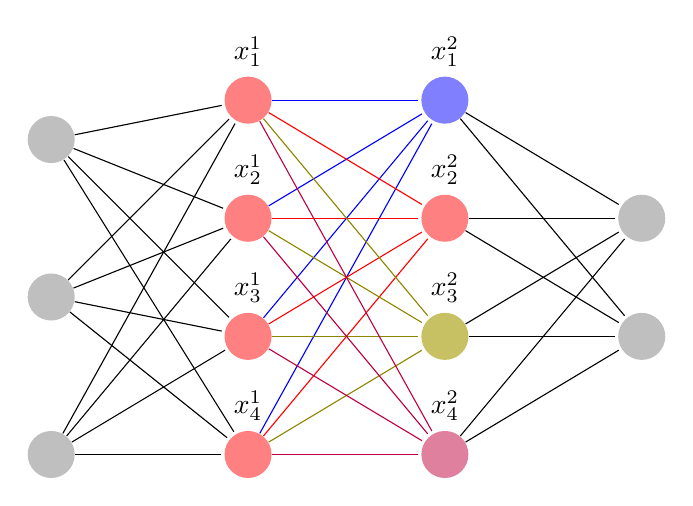
\begin{tikzpicture}[
        >=stealth,
        shorten >=1pt,
        auto,
        node distance=2cm,
        neuron/.style={circle, fill=black!25, minimum size=17pt, inner sep=0pt},
        layer/.style={thick, draw=black!50, rectangle, fill=black!10, minimum height=4em},
    ]
    
        % Draw the input layer nodes
        \foreach \name / \y in {1,...,3}
            \node[neuron] (I-\name) at (0,-\y*2) {};
    
        % Draw the hidden layer nodes
        \foreach \name / \y in {1, ..., 4}
			\node[neuron, fill=red!50, label=above:{$x_{\name}^{1}$}] (H1-\name) at (2.5,-\y*1.5) {};
            
        \foreach \name / \y in {1}
			\node[neuron, fill=blue!50, label=above:{$x_{\name}^{2}$}] (H2-\name) at (5,-\y*1.5) {};
        \foreach \name / \y in {2}
			\node[neuron, fill=red!50, label=above:{$x_{\name}^{2}$}] (H2-\name) at (5,-\y*1.5) {};
        \foreach \name / \y in {3}
			\node[neuron, fill=olive!50, label=above:{$x_{\name}^{2}$}] (H2-\name) at (5,-\y*1.5) {};
        \foreach \name / \y in {4}
			\node[neuron, fill=purple!50, label=above:{$x_{\name}^{2}$}] (H2-\name) at (5,-\y*1.5) {};
    
        % Draw the output layer node
        \foreach \name / \y in {2,3}
            \node[neuron] (O-\name) at (7.5,-\y*1.5) {};
    
        % Connect every node in the input layer with every node in the
        % hidden layer.
        \foreach \source in {1,...,3}
            \foreach \dest in {1,...,4}
                \path (I-\source) edge (H1-\dest);
    
        \foreach \source in {1,...,4}
            \foreach \dest in {1}
				\path (H1-\source) edge[draw=blue] (H2-\dest); 
        \foreach \source in {1,...,4}
            \foreach \dest in {2}
				\path (H1-\source) edge[draw=red] (H2-\dest); 
        \foreach \source in {1,...,4}
            \foreach \dest in {3}
				\path (H1-\source) edge[draw=olive] (H2-\dest); 
        \foreach \source in {1,...,4}
            \foreach \dest in {4}
				\path (H1-\source) edge[draw=purple] (H2-\dest); 
                
        % Connect every node in the hidden layer with the output layer
        \foreach \source in {1,...,4}
            \foreach \dest in {2,3}
                \path (H2-\source) edge (O-\dest);
    \end{tikzpicture}%
\end{minipage}%
\hfill
\begin{minipage}{0.35\textwidth}
    Dato $\mathbf{x}^{0} \in \R^{3}$
    \[
    \mathbf{x}^{1} := \sigma\left( \mathbf{W}_{1} \mathbf{x}^{0} + \mathbf{b}_{1} \right) \in \R^{4}
    \]
    \[
    \mathbf{x}^{2} := \sigma\left( \mathbf{W}_{2} \mathbf{x}^{1} + \mathbf{b}_{2} \right) \in \R^{4}
    \]
    con $\mathbf{W}_{2} \in \R^{4\times 4}$ e $\mathbf{b}\in \R^{4}$.
\end{minipage}
\end{figure}  
\end{frame}


\begin{frame}{Multi-layer Perceptron}
    \begin{figure}
        \begin{minipage}{0.65\textwidth}
    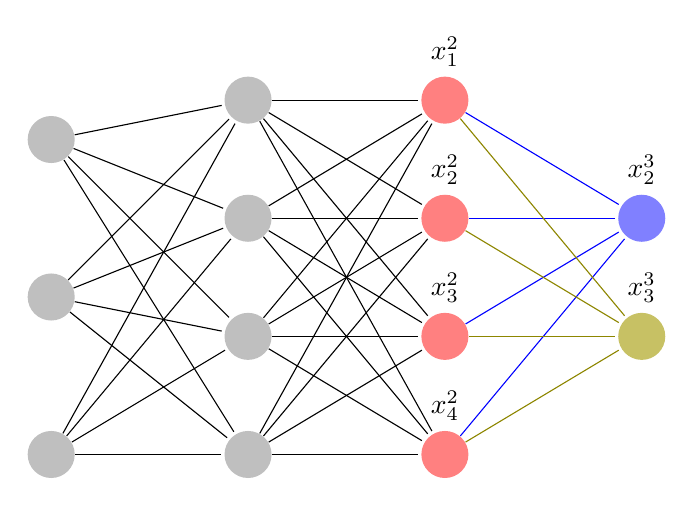
\begin{tikzpicture}[
        >=stealth,
        shorten >=1pt,
        auto,
        node distance=2cm,
        neuron/.style={circle, fill=black!25, minimum size=17pt, inner sep=0pt},
        layer/.style={thick, draw=black!50, rectangle, fill=black!10, minimum height=4em},
    ]
    
        % Draw the input layer nodes
        \foreach \name / \y in {1,...,3}
            \node[neuron] (I-\name) at (0,-\y*2) {};
    
        % Draw the hidden layer nodes
        \foreach \name / \y in {1, ..., 4}
			\node[neuron] (H1-\name) at (2.5,-\y*1.5) {};
            
        \foreach \name / \y in {1, ..., 4}
			\node[neuron, fill=red!50, label=above:{$x_{\name}^{2}$}] (H2-\name) at (5,-\y*1.5) {};
    
        % Draw the output layer node
        \foreach \name / \y in {2}
			\node[neuron, fill=blue!50, label=above:{$x_{\name}^{3}$}] (O-\name) at (7.5,-\y*1.5) {};
        \foreach \name / \y in {3}
			\node[neuron, fill=olive!50, label=above:{$x_{\name}^{3}$}] (O-\name) at (7.5,-\y*1.5) {};
    
        % Connect every node in the input layer with every node in the
        % hidden layer.
        \foreach \source in {1,...,3}
            \foreach \dest in {1,...,4}
                \path (I-\source) edge (H1-\dest);
    
        \foreach \source in {1,...,4}
            \foreach \dest in {1,...,4}
                \path (H1-\source) edge (H2-\dest);
                
        % Connect every node in the hidden layer with the output layer
        \foreach \source in {1,...,4}
            \foreach \dest in {2}
				\path (H2-\source) edge[draw=blue] (O-\dest); 
        \foreach \source in {1,...,4}
            \foreach \dest in {3}
				\path (H2-\source) edge[draw=olive] (O-\dest); 
    \end{tikzpicture}%
\end{minipage}%
\hfill
\begin{minipage}{0.35\textwidth}
    Dato $\mathbf{x}^{0} \in \R^{3}$
    \[
    \mathbf{x}^{1} := \sigma\left( \mathbf{W}_{1} \mathbf{x}^{0} + \mathbf{b}_{1} \right) \in \R^{4}
    \]
    \[
    \mathbf{x}^{2} := \sigma\left( \mathbf{W}_{2} \mathbf{x}^{1} + \mathbf{b}_{2} \right) \in \R^{4}
    \]
    \[
    \mathbf{x}^{3} := \sigma\left( \mathbf{W}_{3} \mathbf{x}^{2} + \mathbf{b}_{3} \right) \in \R^{2}
    \]
    con $\mathbf{W}_{3}\in \R^{2\times 4}$ e $\mathbf{b}\in \R^{2}$.
\end{minipage}
\end{figure}  
\end{frame}

\begin{frame}{Multi-layer Perceptron}
 \begin{definition}{Multi-layer Perceptron}
  Un Multi-layer Perceptron (MLP) con input $\mathbf{x}^{0}\in \R^{d_{0}}$, $L$ hidden layers con $d_{1}, \ldots, d_{L}$ neuroni e output $\mathbf{x}^{L}\in \R^{d_{L}}$ è definito come
    \begin{align*}
     \mathbf{x}^{1} &:= \sigma\left( \mathbf{W}_{1} \mathbf{x}^{0} + \mathbf{b}_{1} \right) \in \R^{d_{1}} \\
     &\vdots \\
     \mathbf{x}^{L} &:= \sigma\left( \mathbf{W}_{L} \mathbf{x}^{L-1} + \mathbf{b}_{L} \right) \in \R^{d_{L}}
    \end{align*}
    dove $\mathbf{W}_{\ell}\in \R^{d_{\ell}\times d_{\ell-1}}$ e $\mathbf{b}_{\ell}\in \R^{d_{\ell}}$ per $\ell=1,\ldots, L$ e $\sigma$ è una funzione di attivazione non lineare applicata componente per componente.
 \end{definition}
\end{frame}

\begin{frame}{Metodo del gradiente}

\end{frame}

\begin{frame}{Convolutional Neural Network (CNN)}
\begin{figure}
    \begin{minipage}{0.7\textwidth}
        \centering
        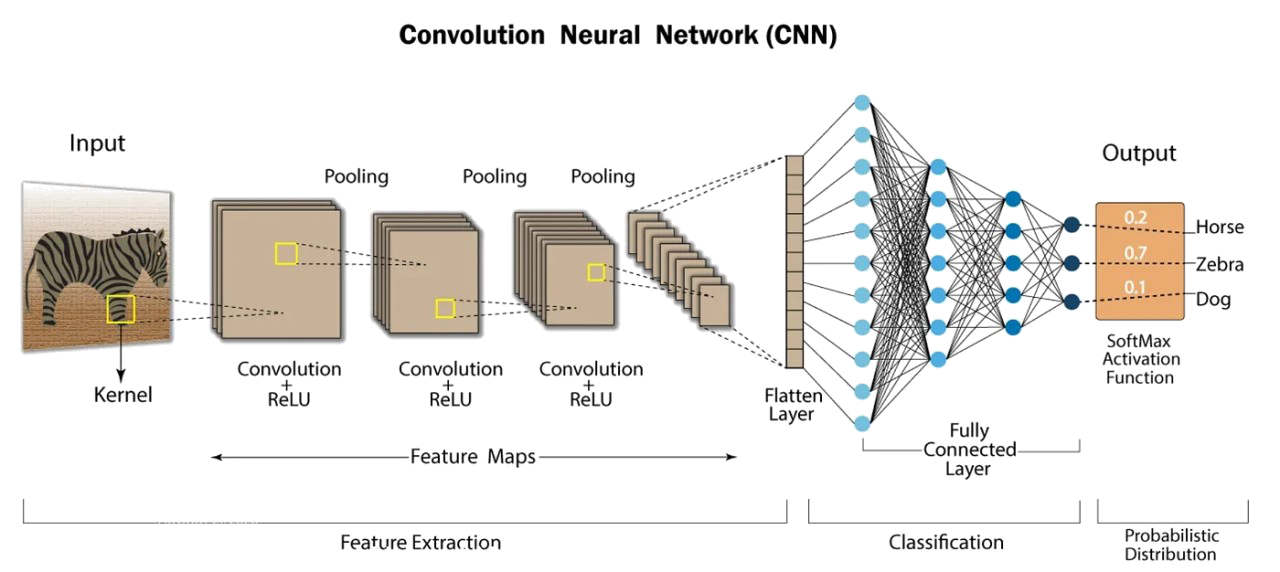
\includegraphics[width=\textwidth]{CNN.png}
    \end{minipage}%
    \begin{minipage}{0.3\textwidth}
        \centering
        Reti neurali convoluzionali per l'applicazione alle immagini.
    \end{minipage}
\end{figure}
\end{frame}

\begin{frame}{Recurrent Neural Network (RNN)}
    \begin{figure}
        \begin{minipage}{0.7\textwidth}
            \centering
            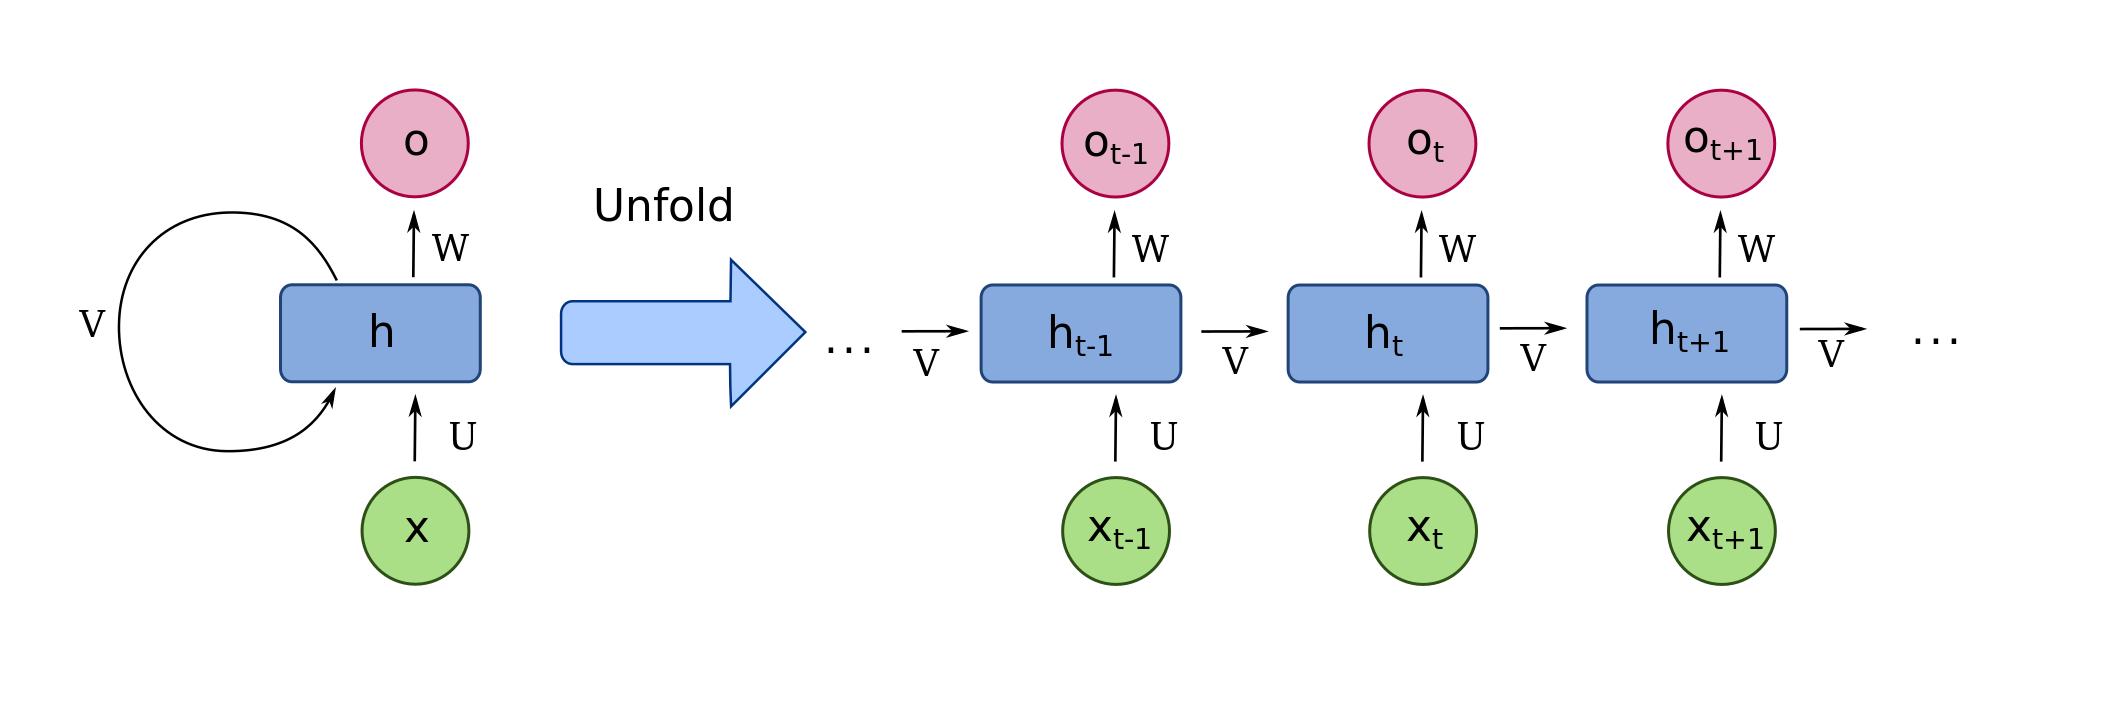
\includegraphics[width=\textwidth]{RNN.png}
        \end{minipage}%
        \begin{minipage}{0.3\textwidth}
            \centering
            Reti neurali ricorrenti per l'applicazione al linguaggio naturale ed ai segnali, o pi\'u in generale alle quantit\'a dipendenti dal tempo.
        \end{minipage}
    \end{figure}
\end{frame}

\begin{frame}{Transformer}
    \begin{figure}
        \begin{minipage}{0.55\textwidth}
            \centering
            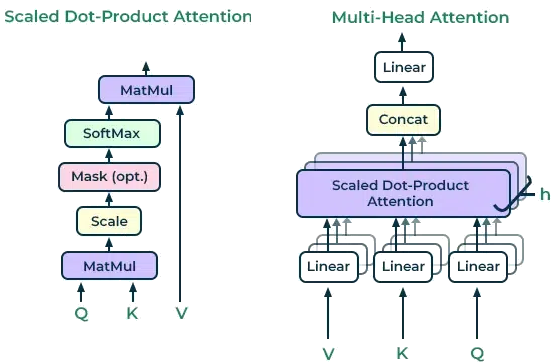
\includegraphics[width=\textwidth]{attention.png}
        \end{minipage}%
        \hfill
        \begin{minipage}{0.3\textwidth}
            \centering
            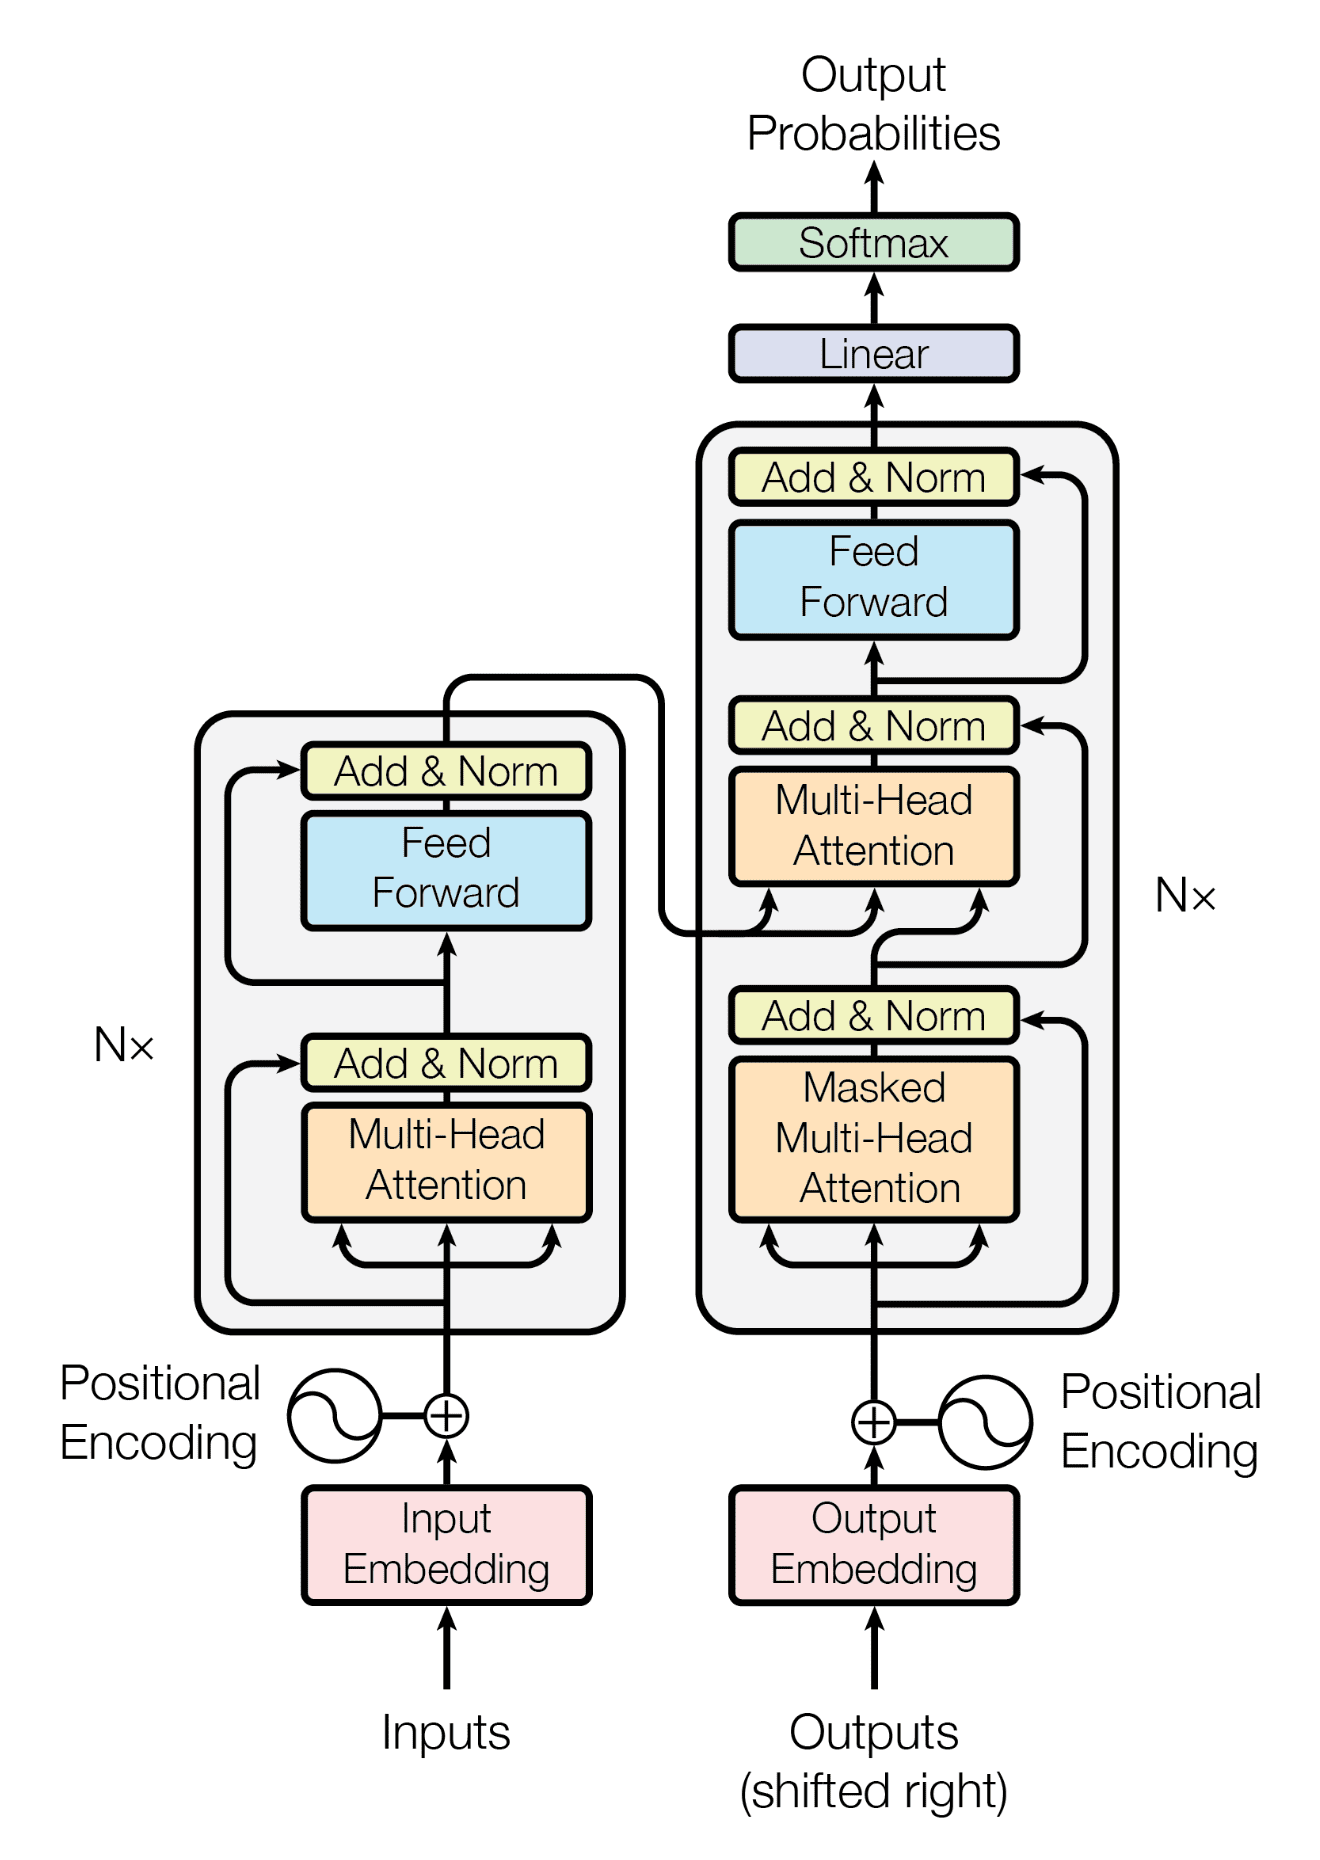
\includegraphics[width=\textwidth]{transformer.png}
        \end{minipage}
    \end{figure}
\end{frame}

\section{Applicazioni interessanti}
\sectionpage


\begin{frame}{Applicazioni alle immagini}
    Siti per generazione d'immagini: \href{https://openai.com/index/dall-e-3/}{DALL-E3} \adjustbox{valign=m}{
\includegraphics[width=1.5cm]{logo-dall-e.png}}, \href{https://www.midjourney.com/home}{Midjourney}  \adjustbox{valign=m}{
\includegraphics[width=0.5cm]{logo-midjourney.png}} e \href{https://ideogram.ai/t/top/1}{Ideogram} \adjustbox{valign=m}{
\includegraphics[width=0.5cm]{logo-ideogram.png}}.
        \begin{center}
            \begin{minipage}{0.23\textwidth}
                
\includegraphics[height=0.7\textheight, width=\textwidth]{ideogram1.png}
            \end{minipage}%
            \hfill
            \begin{minipage}{0.23\textwidth}
                
\includegraphics[height=0.7\textheight, width=\textwidth]{ideogram2.png}
            \end{minipage}%
            \hfill
            \begin{minipage}{0.23\textwidth}
                
\includegraphics[height=0.7\textheight, width=\textwidth]{ideogram4.jpg}
            \end{minipage}%
            \hfill
            \begin{minipage}{0.23\textwidth}
                
\includegraphics[height=0.7\textheight, width=\textwidth]{ideogram3.png}
            \end{minipage}
        \end{center}
\end{frame}

\begin{frame}{Applicazioni ai video}
    Deep learning per la generazione di video \href{https://openai.com/index/sora/}{SORA} \adjustbox{valign=m}{
\includegraphics[width=1.5cm]{logo-sora.png}} o per modificare video anche in tempo reale \href{https://www.nvidia.com/it-it/geforce/broadcasting/broadcast-app/}{NVIDIA Broadcast} \adjustbox{valign=m}{
\includegraphics[width=0.5cm]{logo-broadcast.png}}.
    \vspace{-0.6cm}
    \begin{columns}[T] % align columns
        \begin{column}{.33\textwidth}
            \begin{center}
                % \includemovie[autostart,loop,poster]{0.8\textwidth}{0.7\textheight}{sora1.mp4}
                \movie[externalviewer]{
\includegraphics[width=0.8\textwidth]{sora1-img.png}}{sora1.mp4}
            \end{center}
        \end{column}%
        \begin{column}{.33\textwidth}
            \begin{center}
                % \includemovie[autostart,loop,poster]{0.8\textwidth}{0.7\textheight}{sora2.mp4}
                \movie[externalviewer]{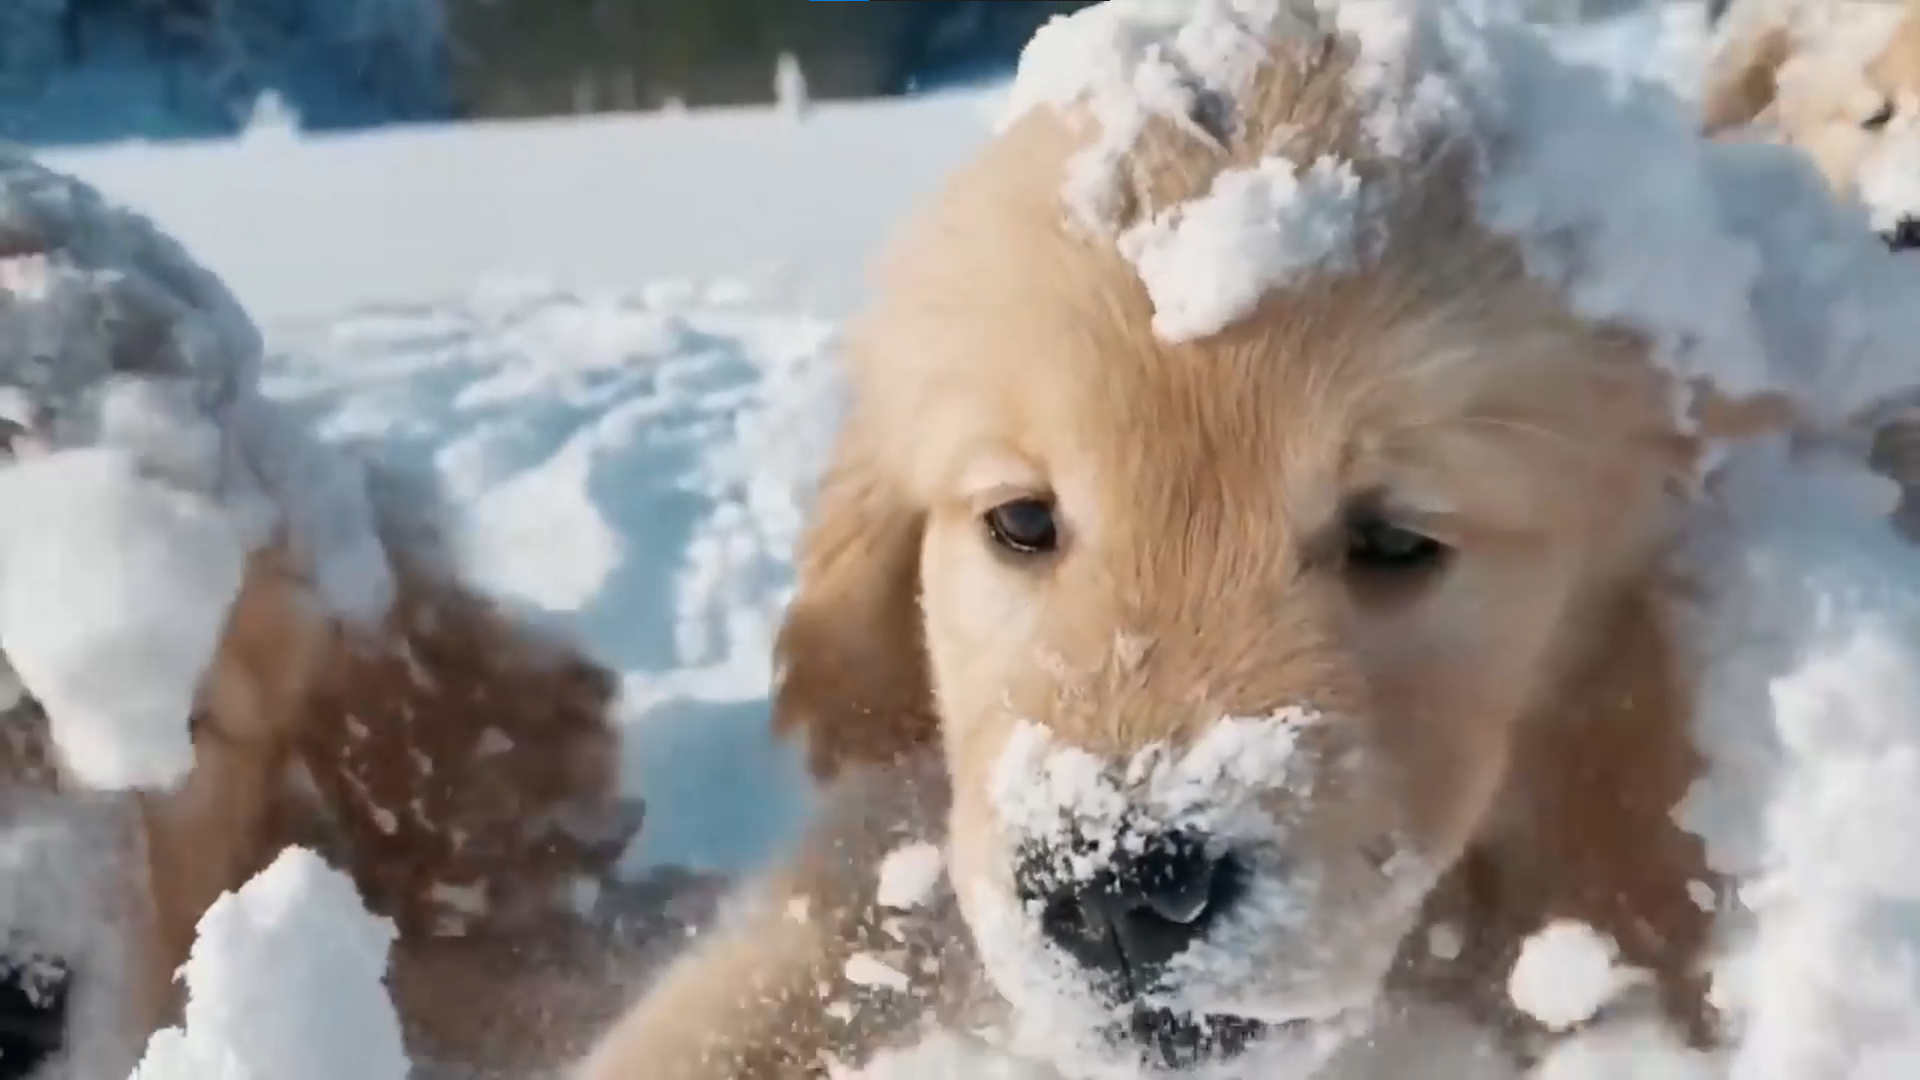
\includegraphics[width=0.8\textwidth]{sora2-img.png}}{sora2.mp4}
            \end{center}
        \end{column}%
        \begin{column}{.33\textwidth}
            \begin{center}
                % \includemovie[autostart,loop,poster]{0.8\textwidth}{0.7\textheight}{sora5.mp4}
                \movie[externalviewer]{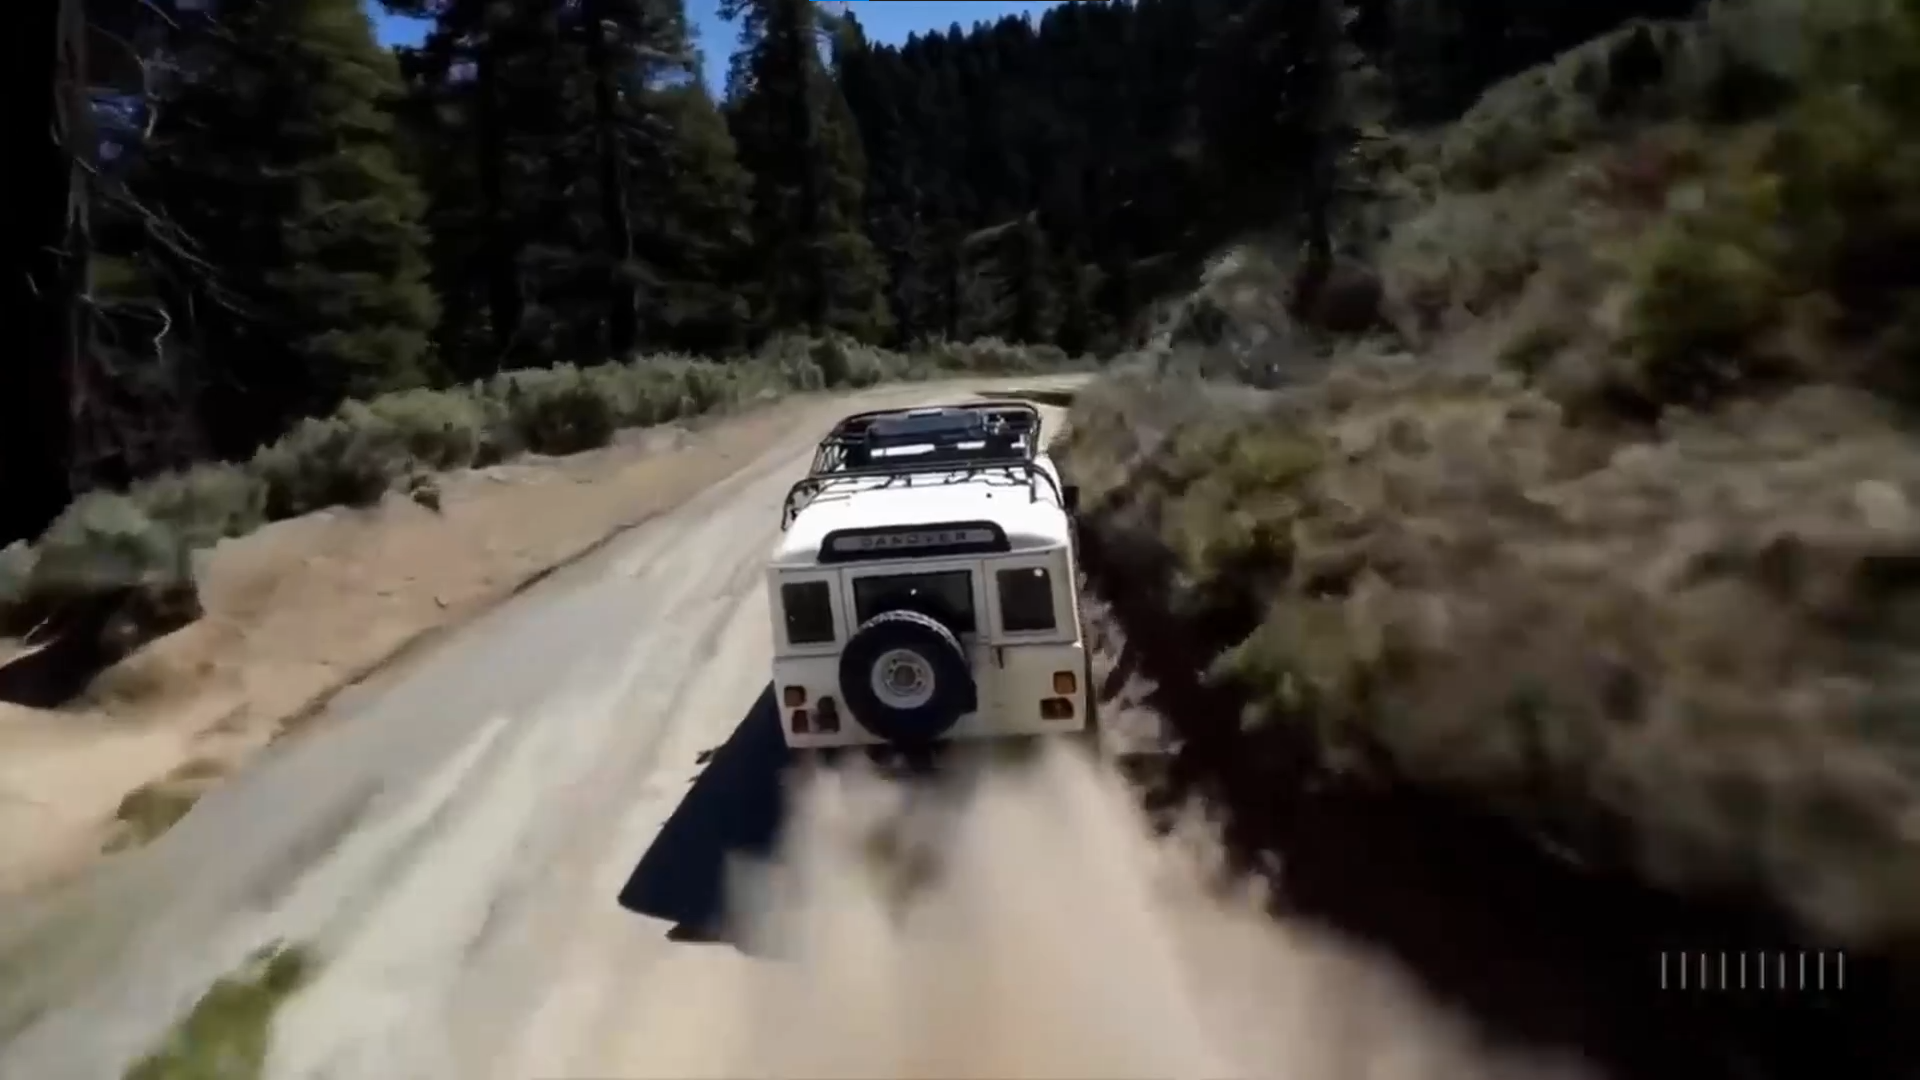
\includegraphics[width=0.8\textwidth]{sora5-img.png}}{sora5.mp4}
            \end{center}
        \end{column}
    \end{columns}

    \begin{columns}[T] % align columns
        \begin{column}{.33\textwidth}
            \begin{center}
                % \includemovie[autostart,loop,poster]{0.8\textwidth}{0.7\textheight}{sora3.mp4}
                \movie[externalviewer]{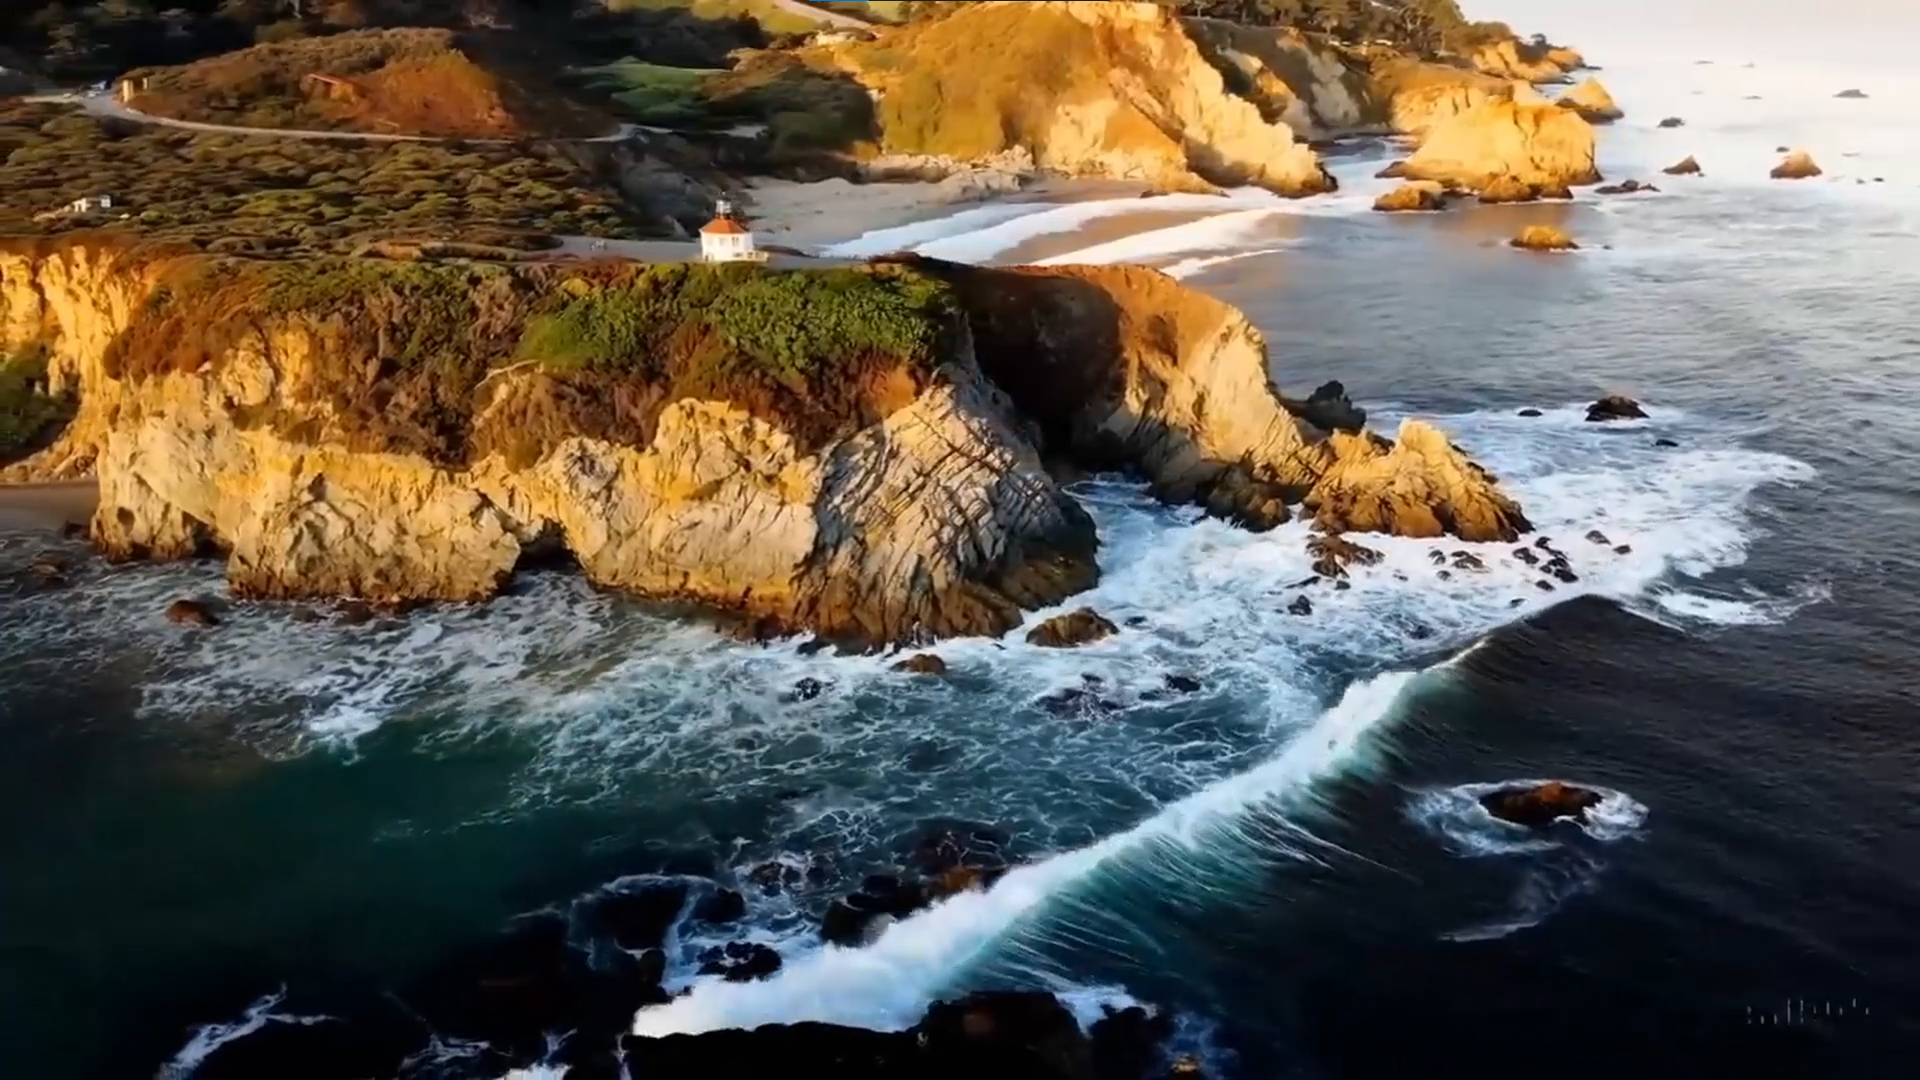
\includegraphics[width=0.8\textwidth]{sora3-img.png}}{sora3.mp4}
            \end{center}
        \end{column}%
        \begin{column}{.33\textwidth}
            \begin{center}
                % \includemovie[autostart,loop,poster]{0.8\textwidth}{0.7\textheight}{sora4.mp4}
                \movie[externalviewer]{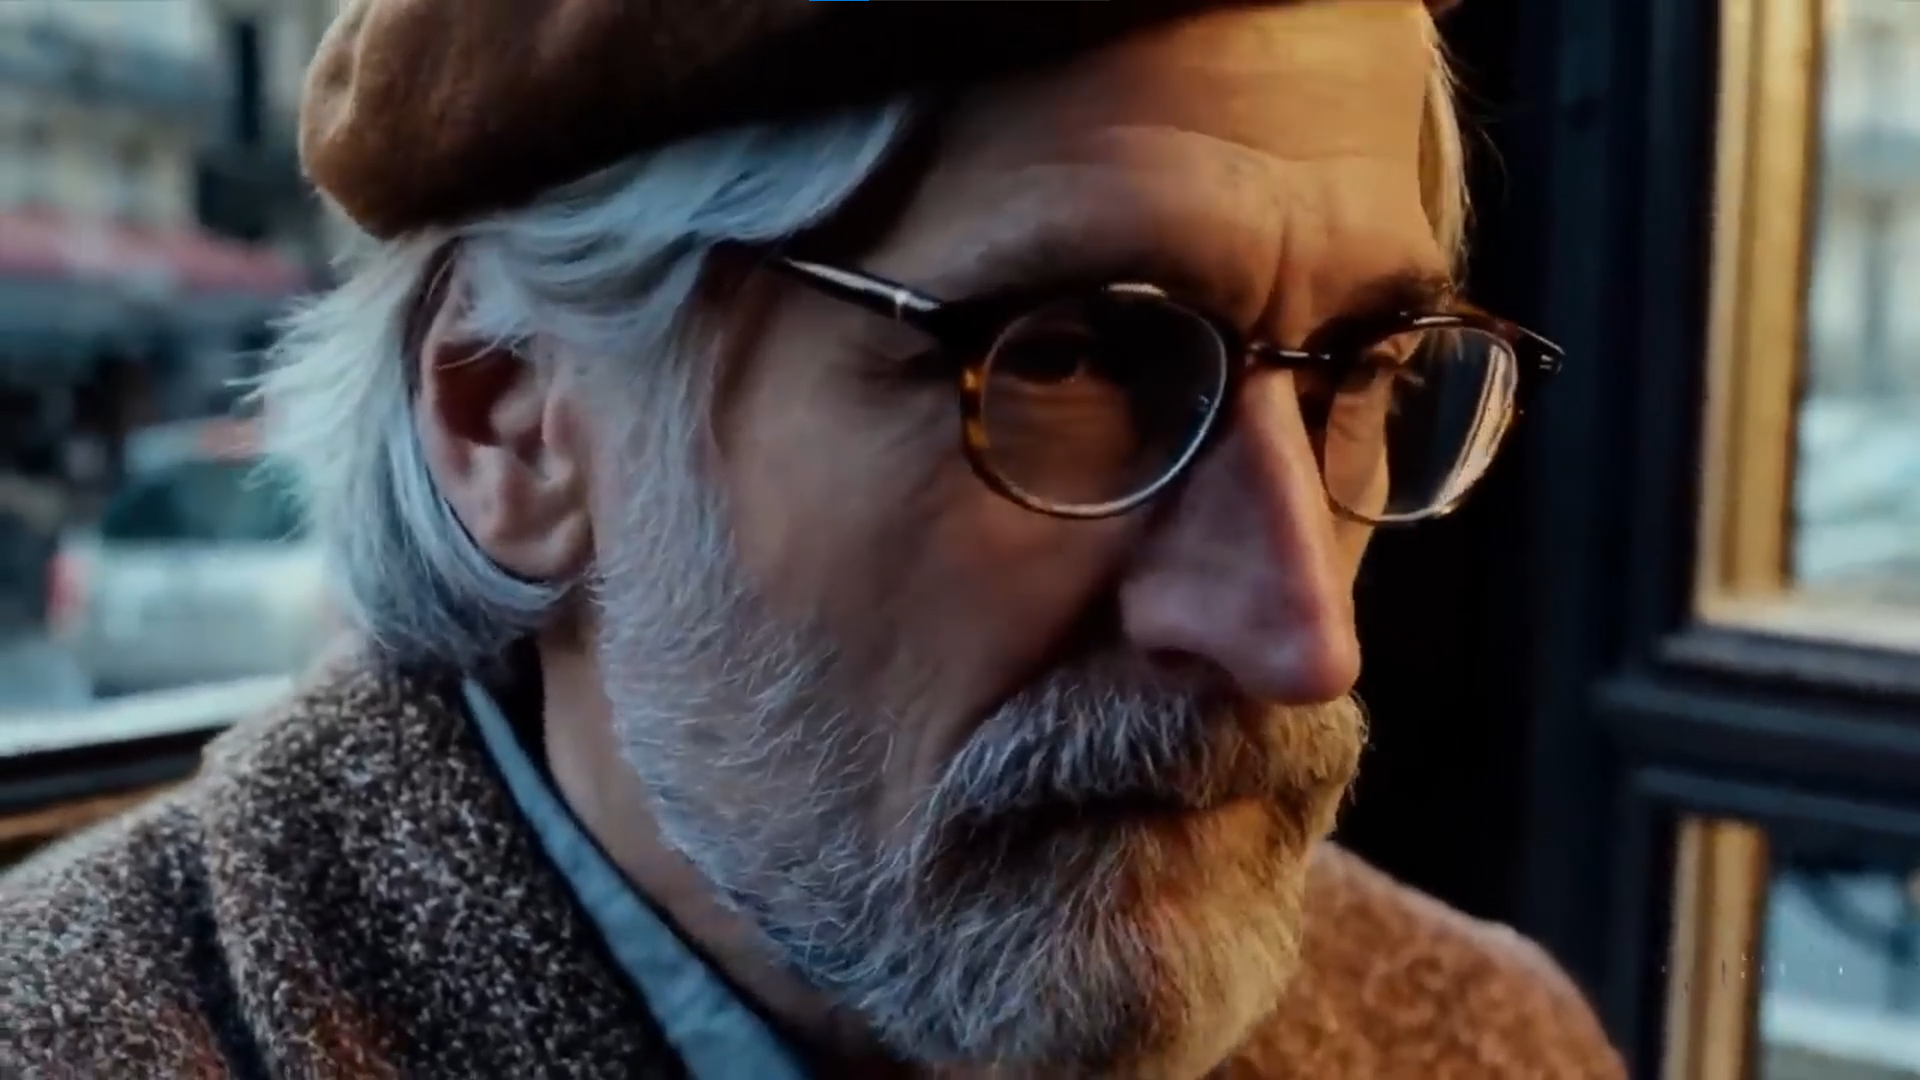
\includegraphics[width=0.8\textwidth]{sora4-img.png}}{sora4.mp4}
            \end{center}
        \end{column}%
        \begin{column}{.33\textwidth}
            \begin{center}
                % \includemovie[autostart,loop,poster]{0.8\textwidth}{0.7\textheight}{sora6.mp4}
                \movie[externalviewer]{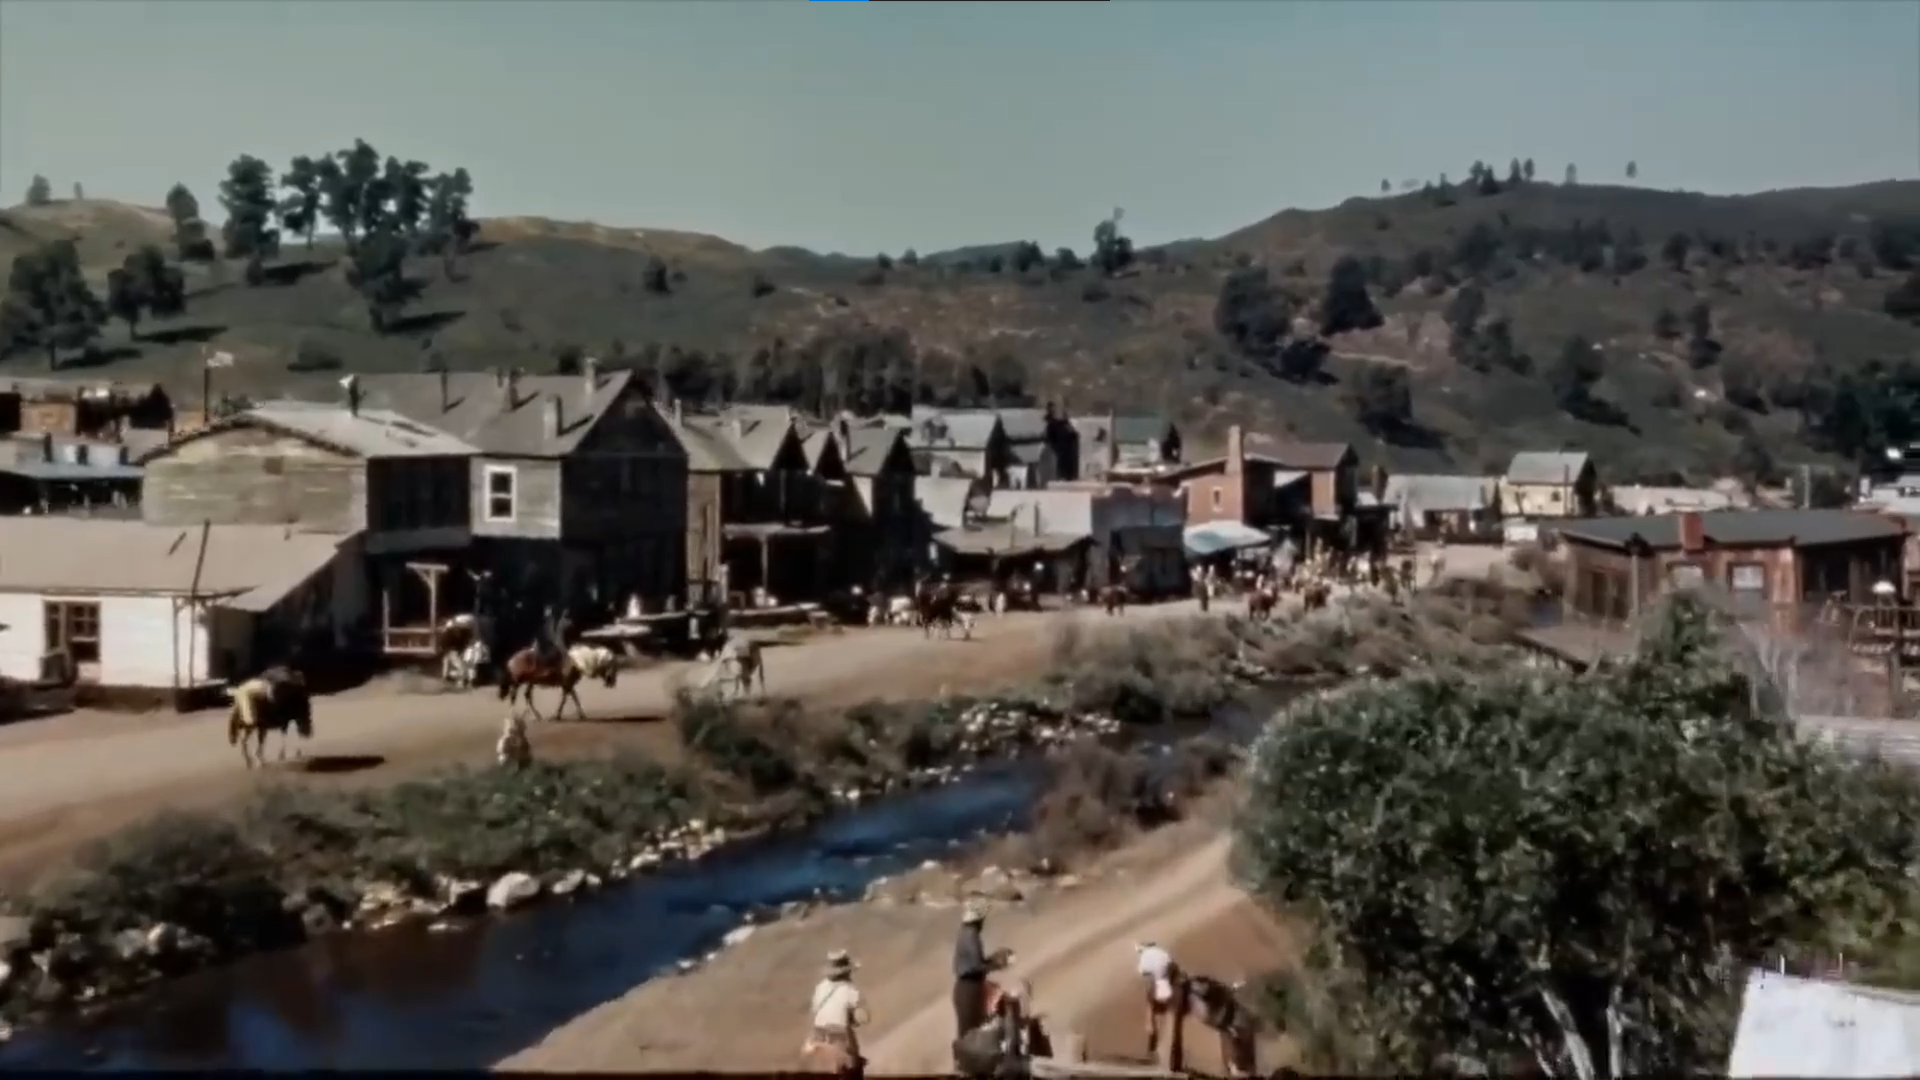
\includegraphics[width=0.8\textwidth]{sora6-img.png}}{sora6.mp4}
            \end{center}
        \end{column}
    \end{columns}
\end{frame}

\begin{frame}{Applicazioni al linguaggio}
    \begin{itemize}
    \item Modelli per la generazione di testo come \href{https://openai.com/index/gpt-4/}{GPT-4} \adjustbox{valign=m}{
\includegraphics[width=1.5cm]{logo-chat-gpt4.png}} o \href{https://github.com/features/copilot}{Copilot} \adjustbox{valign=m}{
\includegraphics[width=0.5cm]{logo-copilot.png}}.
    \item Esistono modelli open-source come \href{https://llama.meta.com/}{LLaMA-3} \adjustbox{valign=m}{
\includegraphics[width=1.5cm]{logo-llama.png}} scaricabile graatuitamente dal loro sito. 
    \end{itemize}
    \pause
    Per allenare Chat-GPT3, formata da $175$ bilioni di parametri, hanno impiegato $1023$ Nvidia A$100$ per $34$ giorni spendendo $5$ milioni di dollari in corrente.
    
    \pause
    Anche per scaricare il modello più piccolo di LLaMA $3$ $8B$ sono necessari $20$ GB di VRAM e per il modello $LLaMA$ $3$ $70B$ sono necessari $140GB$ di spazio e $160GB$ di VRAM in $FP16$.
\end{frame}

\section{Operatori neurali}
\sectionpage

\begin{frame}{Deep Operator Network}
\begin{center}
    \begin{tikzpicture}
        \node (branch) [label={[font=\footnotesize]left:$\mathbf{f}_i = \begin{bmatrix} f_i(x_1) \\ \vdots \\ f_i(x_m) \end{bmatrix} \in \R^m$}, label={[font = \small]above:Branch Network}, font=\footnotesize]{
            \begin{tikzpicture}[
            >=stealth,
            shorten >=1pt,
            auto,
            node distance=2cm,
            neuron/.style={circle, fill=orange!25, minimum size=7pt, inner sep=0pt},
            layer/.style={thick, draw=black!50, rectangle, fill=black!10, minimum height=4em},
        ]
            \def\altezza{0.5};
            \def\larghezza{1};
            % Draw the input layer nodes
            \foreach \name / \y in {1,...,3}
                \node[neuron] (I-\name) at (0,-\y*\altezza-\altezza/2) {};
        
            % Draw the hidden layer nodes
            \foreach \name / \y in {1,...,4}
                \node[neuron] (H1-\name) at (\larghezza,-\y*\altezza) {};
                
            \foreach \name / \y in {1,...,4}
                \node[neuron] (H2-\name) at (\larghezza*2,-\y*\altezza) {};
        
            % Draw the output layer node
            \foreach \name / \y in {2,3}
                \node[neuron] (O-\name) at (\larghezza*3,-\y*\altezza) {};
        
            % Connect every node in the input layer with every node in the
            % hidden layer.
            \foreach \source in {1,...,3}
                \foreach \dest in {1,...,4}
                    \path (I-\source) edge (H1-\dest);
                    
            \foreach \source in {1,...,4}
                \foreach \dest in {1,...,4}
                    \path (H1-\source) edge (H2-\dest);
        
            % Connect every node in the hidden layer with the output layer
            \foreach \source in {1,...,4}
                \foreach \dest in {2,3}
                    \path (H2-\source) edge (O-\dest);
        \end{tikzpicture}%
        };%
        \node[below=0.5cm of branch, label={[font=\footnotesize]left:$\mathbf{y} = \begin{bmatrix} y_1 \\ \vdots \\ y_d \end{bmatrix} \in \Omega    \subset \R^d$}, label={[font=\small]below:Trunk Network}, font=\footnotesize] (trunk) {
        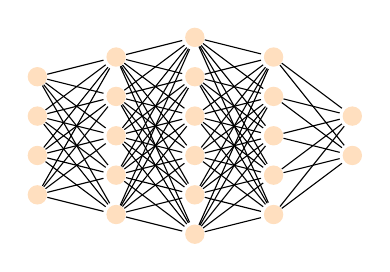
\begin{tikzpicture}[
            >=stealth,
            shorten >=1pt,
            auto,
            node distance=2cm,
            neuron/.style={circle, fill=orange!25, minimum size=7pt, inner sep=0pt},
            layer/.style={thick, draw=black!50, rectangle, fill=black!10, minimum height=4em},
            % node_prod/.style={draw, circle, fill=white, inner sep=0pt, minimum size=6mm},
        ]
            \def\altezza{0.5};
            \def\larghezza{1};
            % Draw the input layer nodes
            \foreach \name / \y in {1,...,4}
                \node[neuron] (I-\name) at (0,-\y*\altezza) {};
        
            % Draw the hidden layer nodes
            \foreach \name / \y in {1,...,5}
                \node[neuron] (H1-\name) at (\larghezza,-\y*\altezza + \altezza/2) {};
                
            \foreach \name / \y in {1,...,6}
                \node[neuron] (H2-\name) at (\larghezza*2,-\y*\altezza + \altezza) {};
        
            \foreach \name / \y in {1,...,5}
                \node[neuron] (H3-\name) at (\larghezza*3,-\y*\altezza + \altezza/2) {};

            % Draw the output layer node
            \foreach \name / \y in {2,3}
                \node[neuron] (O-\name) at (\larghezza*4,-\y*\altezza) {};
        
            % Connect every node in the input layer with every node in the
            % hidden layer.
            \foreach \source in {1,...,4}
                \foreach \dest in {1,...,5}
                    \path (I-\source) edge (H1-\dest);
                    
            \foreach \source in {1,...,5}
                \foreach \dest in {1,...,6}
                    \path (H1-\source) edge (H2-\dest);
        
            \foreach \source in {1,...,6}
                \foreach \dest in {1,...,5}
                    \path (H2-\source) edge (H3-\dest);

            % Connect every node in the hidden layer with the output layer
            \foreach \source in {1,...,5}
                \foreach \dest in {2,3}
                    \path (H3-\source) edge (O-\dest);
        \end{tikzpicture}%
    };%
    \node (middle) at ($($(branch.east)+(1, 0)$)!0.5!($(trunk.east)+(1, 0)$)$) {}; % middle node
    \draw[->] (branch.east) -- ($(middle.north)-(0.1, -0.1)$); % arrow from the end of the first diagram
    \draw[->] (trunk.east) -- ($(middle.south)-(0.1, 0.1)$); % arrow from the end of the second diagram
    \node[draw, circle, fill=white, inner sep = 0pt, minimum size = 4mm, font = \footnotesize] (node_prod) at (middle) {$\times$};
    \node (label) at ($(middle)+(1,0)$) [label=right:{$\mathcal{G}(\mathbf{f}_i)(\mathbf{y})$}, font=\footnotesize] {}; % define the label node
    \draw[->] ($(middle.east)+(0.15, 0)$) -- ($(label)+(0.2, 0)$); % draw an arrow from the middle node to the label node
    \end{tikzpicture}
\end{center}
\end{frame}

\begin{frame}{Fourier Neural Operator}
    \begin{center}
    \begin{tikzpicture}
        \tikzset{
            box/.style={draw, rounded corners, align=center, minimum height=0.8cm, minimum width=1cm, fill=orange!30},
            bigbox/.style={draw, rounded corners, align=center, minimum height=2cm, minimum width=1cm, fill=yellow!30},
            node_sum/.style={draw, circle, fill=white, inner sep=0pt, minimum size=4mm},
            every node/.style={font=\small}
        }
        % Nodes for the main structure
        \node[box, label=above:{\textit{Input}}] (input) {$f(x)$};
        \node[box, right=0.5cm of input, label=above:{\textit{Lifting}}] (lifting) { $\mathcal{P}$ };
        \node[bigbox, right=0.5cm of lifting] (fourier1) {$\mathcal{L}_{1}$};
        \node[bigbox, right=0.55cm of fourier1] (fourier2) {$\mathcal{L}_{t}$};
        \node[bigbox, right=0.55cm of fourier2] (fourier3) {$\mathcal{L}_{L}$};
        \node[box, right=0.5cm of fourier3, label=above:{\textit{Projection}}] (projection) {$\mathcal{Q}$};
        \node[box, right=0.5cm of projection, label=above:{\textit{Output}}] (output) {$u(x)$};
        
        % Draw arrows between nodes
        \draw[->, line width = .7pt] ($(input.east)+(0.05, 0)$) -- ($(lifting.west)-(0.05,0)$);
        \draw[->, line width = .7pt] ($(lifting.east)+(0.05, 0)$) -- ($(fourier1.west)-(0.03,0)$);
        \draw[dotted, line width = 2pt] ($(fourier1.east)+(0.1, 0)$) -- ($(fourier2.west)-(0.1,0)$);
        \draw[dotted, line width = 2pt] ($(fourier2.east)+(0.1, 0)$) -- ($(fourier3.west)-(0.1,0)$);
        \draw[->, line width = .7pt] ($(fourier3.east)+(0.05, 0)$) -- ($(projection.west)-(0.05,0)$);
        \draw[->, line width = .7pt] ($(projection.east)+(0.05, 0)$) -- ($(output.west)-(0.05,0)$);
        
        % Annotations for the Fourier Layers
        \node[align=center, above=0.2cm of fourier2, font=\footnotesize] { \textit{Fourier Layers} };
        
        % Internal structure bounding box
        \node[draw, line width = .7pt, rounded corners, inner sep=0.15cm, fit= (fourier1) (fourier2) (fourier3)] (internal) {};

        %%% Second part of the plot
        % Internal structure bounding box
		\node[draw, below=0.2cm of internal, rounded corners, inner sep=0.2cm, fill=yellow!30] (internal) {
			\begin{tikzpicture}[every node/.style={font=\small}]
				% Nodes for the internal structure
				\node[box] (vt) {$v_{t}(x)$};
				\node[box, right=1cm of vt] (transform) {$\mathcal{F}$};
				\node[box, right=0.5cm of transform, fill=green!25] (nonlinear) { $ R_{\theta_t} $ };
				\node[box, right=0.5cm of nonlinear] (invtransform) { $ \mathcal{F}^{-1} $ };
				\node[box, below=0.8cm of nonlinear, fill=green!25] (linear) { $ W_t, b_t $ };

                % Internal structure bounding box
                \node[draw, line width = .7pt, rounded corners, inner sep=0.15cm, fit= (transform) (nonlinear) (invtransform) ] (diagonalscaling) {};

				\node[node_sum, right=0.5cm of invtransform] (node_sum) {$\mathbf{+}$};
				\node[box, right=0.5cm of node_sum] (activation) {$\sigma$};
				\node[box, right=0.5cm of activation] (vtplusone) {$v_{t+1}(x)$};
				
				% Draw arrows between nodes
				\draw[line width = .7pt] ($(vt.east)+(0.05, 0)$) -- (diagonalscaling);
				\draw[->, line width = .7pt] ($(transform.east)+(0.05, 0)$) -- ($(nonlinear.west)-(0.05, 0)$);
				\draw[->, line width = .7pt] ($(nonlinear.east)+(0.05, 0)$) -- ($(invtransform.west)-(0.05, 0)$);
				\draw[->, line width = .7pt] ($(vt.south)-(0, 0.05)$) |- ($(linear.west)-(0.05, 0)$);
				\draw[->, line width = .7pt] (diagonalscaling) -- ($(node_sum.west)-(0.05, 0)$);
				\draw[->, line width = .7pt] ($(linear.east)+(0.05, 0)$) -| ($(node_sum.south)-(0, 0.05)$);
				\draw[->, line width = .7pt] ($(node_sum.east)+(0.05, 0)$) -- ($(activation.west)-(0.05, 0)$);
				\draw[->, line width = .7pt] ($(activation.east)+(0.05, 0)$) -- ($(vtplusone.west)-(0.05, 0)$);

			\end{tikzpicture}
		};
        % Connection between the two parts
        \draw[] ($(internal.north west)+(0.1, 0.05)$) -- (fourier2.south west);
        \draw[] ($(internal.north east)+(-0.1, 0.05)$) -- (fourier2.south east);
    \end{tikzpicture}
    \end{center}
\end{frame}

\section{Approsimazione di equazioni differenziali}
\sectionpage
	
\end{document}

Titolo: Operatori neurali
Sottotitolo: machine learning per matematici

ABSTRACT OF THE TALK HERE:
Negli ultimi anni, il campo dell'intelligenza artificiale ha subito una notevole evoluzione, con applicazioni sempre più diffuse in una vasta gamma di settori. Questo seminario si propone di esplorare tale evoluzione attraverso due principali argomenti. Nella prima parte, sarà presentata una panoramica del Deep Learning, evidenziando le architetture chiave e illustrando diverse applicazioni di rilievo. Successivamente, ci concentreremo sulla teoria fondamentale del machine learning, introducendo il concetto di operatori neurali e esaminando la loro utilità nell'approssimazione di soluzioni per equazioni differenziali. Attraverso esempi pratici, sarà mostrato come tali operatori possano contribuire in modo significativo alla risoluzione di problemi complessi.

\begin{frame}
	\onslide<1->{}
	\onslide<2->{}
	\onslide<3->{}
\end{frame}

\section{}
\sectionpage

\begin{theorem}
\end{theorem}